%%%%%%%%%%%%%%%%%%%%%%%%%%%%%%%%%%%%%%%%%%%%%%%%%%%%%%%%%%%%%%%%%%%%%%%
% Universidade Federal de Santa Catarina             
% Biblioteca Universitária                     
%----------------------------------------------------------------------
% Exemplo de utilização da documentclass ufscThesis
%----------------------------------------------------------------------                                                           
% (c)2013 Roberto Simoni (roberto.emc@gmail.com)
%         Carlos R Rocha (cticarlo@gmail.com)
%         Rafael M Casali (rafaelmcasali@yahoo.com.br)
%%%%%%%%%%%%%%%%%%%%%%%%%%%%%%%%%%%%%%%%%%%%%%%%%%%%%%%%%%%%%%%%%%%%%%%
\documentclass{ufscThesis} % Definicao do documentclass ufscThesis	

%----------------------------------------------------------------------
% Pacotes usados especificamente neste documento
%\usepackage[utf8]{inputenc}
%\usepackage[T1]{fontenc}
\usepackage{graphicx} % Possibilita o uso de figuras e gráficos
\usepackage{color}    % Possibilita o uso de cores no documento
\usepackage{pdfpages} % Possibilita a inclusão da ficha catalográfica
\usepackage{listings}
\usepackage{float}
\usepackage{fancyhdr}
\usepackage{subcaption}
\usepackage{pgfplots}
\usepgfplotslibrary{units}
\usepackage{array}
\usepackage{listings}
\usepackage{import}
\usepackage{amsmath}
\usepackage{sagetex}
\usepackage{subfig}
\usepackage{amsmath}%
\usepackage{MnSymbol}%
\usepackage{wasysym}%
\usepackage{filecontents}
\usepackage{lscape}
\usepackage[decimalsymbol=comma]{siunitx}
\pgfplotsset{width=.9\linewidth,compat=1.9}


%----------------------------------------------------------------------
% Comandos criados pelo usuário
\newcommand{\afazer}[1]{{\color{red}{#1}}} % Para destacar uma parte a ser trabalhada
\newcommand{\ABNTbibliographyname}{REFERÊNCIAS} % Necessário para abnTeX 0.8.2


%----------------------------------------------------------------------
% Identificadores do trabalho
% Usados para preencher os elementos pré-textuais
\instituicao[a]{Universidade Federal de Santa Catarina} % Opcional
\departamento[a]{Departamento de Engenharia Mecânica}
\curso[o]{Programa de Pós-Graduação}
\documento[o]{Dissertação} % [o] para dissertação [a] para tese
\titulo{Ferramenta Computacional para Análise da Acústica Interna de Dutos}
\subtitulo{} % Opcional
\autor{José Pedro de Santana Neto}
\grau{Mestre em Engenharia Mecânica}
\local{Florianópolis} % Opcional (Florianópolis é o padrão)
\data{15}{Agosto}{2017}
\orientador[Orientador]{Andrey Ricardo da Silva, Ph.D.}
%\coorientador[Coorientador]{Henrique Simas, Dr. Eng.}
\coordenador[Coordenador]{Jonny Carlos da Silva, Dr. Eng.}

\numerodemembrosnabanca{2} % Isso decide se haverá uma folha adicional
\orientadornabanca{nao} % Se faz parte da banca definir como sim
\coorientadornabanca{nao} % Se faz parte da banca definir como sim
\bancaMembroA{Júlio Apolinário Cordioli, Dr. Eng.\\Universidade Federal de Santa Catarina} %Nome do presidente da banca
\bancaMembroB{Luis Orlando Emerich dos Santos, Dr. Eng.\\Universidade Federal de Santa Catarina}      % Nome do membro da Banca
\bancaMembroC{Arcanjo Lenzi, Ph.D.\\Universidade Federal de Santa Catarina}     % Nome do membro da Banca
\bancaMembroD{Quarto membro\\Universidade ...}       % Nome do membro da Banca
%\bancaMembroE{Quinto membro\\Universidade ...}       % Nome do membro da Banca
%\bancaMembroF{Sexto membro\\Universidade ...}        % Nome do membro da Banca
%\bancaMembroG{Sétimo membro\\Universidade ...}       % Nome do membro da Banca

\dedicatoria{Este trabalho é dedicado às pessoas que possuem a estranha mania de ter fé na vida.}

\agradecimento{Agradeço primeiramente a Deus, por permitir-me nesse mundo, vivendo, aprendendo e contemplando a beleza da natureza primordial de todas as coisas.

A minha amada e querida mãe Francisca, pela paciência, compreensão, tolerância, conselhos, carinho, dedicação, afeto, amizade, silêncio, sorrisos e um intenso amor. Meu primeiro aprendizado na vida mais puro e original de amor foi através dela. Meus sinceros e eternos agradecimentos.

A meu pai Luciano, mesmo não estando presente mais, me inspirou a escolha da minha formação e me ensinou a olhar o mundo com meus próprios olhos.

A meu irmão João, companheiro e amigo de sempre. Seus conselhos e seu exemplo têm me ensinado muito a ser uma pessoa melhor.

A minha amada e querida namorada Simone, pelo companheirismo, amizade, carinho, afeto, conselhos, paciência e sobretudo muito amor. Infinitamente agradecido por tudo.  

A meu padrinho Inácio, meu tio Antônio, minha madrinha Nevinha, minhas tias Titia e Tia Marli por seus profundos conselhos sobre a vida, apoio, carinho e amor. A toda minha família pelo apoio, confiança e compressão.

A meus amigos de Brasília Thiago, Leandro, Vilmey, Yan e Henrique pelo companheirismo indescritível de muitos anos e apoio de sempre.

A meu orientador professor Andrey, pelo exemplo, inspiração, conselhos, apoio, confiança e investimento de longas conversas. Esse trabalho necessariamente foi fruto de longas horas de esforço e trabalho em conjunto.

Aos professores Júlio e Arcanjo (Chefe), pelos valiosos ensinamentos e exemplos de profissionais-cientistas.

Aos meus amigos de Florianópolis Wagner, Danilo, Matheus, Luisa, André Spillere, André Loch, Zargos, Gil, Caetano, Giordano e o pessoal do GOJ e outros que esqueci de citar pela compreensão, apoio e motivação.

A equipe do LVA e da pós-graduação em Engenharia Mecânica pelo suporte e aprendizado na produção científica.

E as pessoas que passaram na minha vida e influenciaram de alguma forma nesse trabalho. Meus agradecimentos.
}

\epigrafe{Muitos acham que o som é um corpo rígido vibrando, mas o som é fluido assim como a vida.}
{(José Pedro de Santana Neto, 2017)}

\textoResumo {Analisar e estudar acústica de dutos na presença de fluxo de massa vem se tornado um desafio visto que a interação entre esses dois fenômenos afeta significativamente o comportamento acústico. Estudos investigativos matemáticos ou experimentais podem ser inviáveis nesse sentido devido a complexidade matemática ou altos custos de bancada e, para contornar esse problema, faz-se o uso de métodos numéricos e tecnologias computacionais. Nesse trabalho é desenvolvido e validado uma ferramenta computacional para análise do coeficiente de reflexão para modos normais em dutos na presença de escoamentos de baixo número de Mach ($M \leq 0,2$). Para tal foi utilizado o método de \textit{lattice} Boltzmann e suas condições de contorno implementados no software livre Palabos, bem como constiuído um modelo numérico tridimensional de um duto não flangeado. Foram abordados as condições sem escoamento, com escoamento de exaustão e com escoamento succionado para validar a ferramenta computacional, resultando em boas concordâncias com a literatura vigente, além de propiciar mais informações sobre regimes de succção no que diz respeito interação de vórtices com o campo acústico.}
\palavrasChave {Aeroacústica. Ferramenta Computacional. Acústica Interna de Dutos. Método de \textit{lattice} Boltzmann. Palabos. Coeficiente de Reflexão.}
 
\textAbstract {Analyzing and studying duct acoustics in the presence of mass flow has become a challenge since the interaction between these two phenomena significantly affects the acoustic behavior. Mathematical or experimental investigative studies may be impracticable in this sense due to mathematical complexity or high bench costs and, to overcome this problem, numerical methods and computational technologies are used. In this work a computational tool for analysis of the reflection coefficient for normal modes in ducts in the presence of low Mach number flows ($M \leq 0.2$) is developed and validated. The lattice Boltzmann method and its boundary conditions implemented in the free software Palabos were used as well as a three-dimensional numerical model of a non-flanged duct. The non-flowing, out flow and inlet flow conditions were addressed to validate the computational tool, resulting in good agreement with the current literature, as well as providing more information on suction regimes with respect to vortex interaction with the acoustic field.}
\keywords {Aeroacoustics. Computational Tool. Internal Acoustics of Pipelines. Lattice Boltzmann Method. Palabos. Coefficient of Reflection.}

%----------------------------------------------------------------------
% Início do documento                                
\usepackage{comandos}

\begin{document}
%--------------------------------------------------------
% Elementos pré-textuais
\capa  
\folhaderosto[comficha] % Se nao quiser imprimir a ficha, é só não usar o parâmetro
\folhaaprovacao
\paginadedicatoria
\paginaagradecimento
\paginaepigrafe
\paginaresumo
\paginaabstract
%\pretextuais % Substitui todos os elementos pre-textuais acima
\listadefiguras % as listas dependem da necessidade do usuário
\listadetabelas 
\listadeabreviaturas
\listadesimbolos
%%%%%%
%\f
\sumario
%--------------------------------------------------------
% Elementos textuais
%%%%%%%%%%%%%%%%%%%%%%%%%%%%%%%%%%%%%%%%%%%%%%%%%%%%%%%%%%%%%%%%%%%%%%%%

\chapter{Introdução}
\label{chapter:introdcao}

\section{Contexto}

% Falar sobre sistemas de exaustão com exemplos
Sistemas de fluxo de massa (exaustão e sucção) podem se tornar uma considerável fonte de ruído. Escapamentos, sistemas de ventilação, buzinas, motores aeronáuticos e aspiradores de pó são exemplos desses sistemas que estão altamente presentes no dia-a-dia. Cada vez mais, a sociedade vem desenvolvendo consciência crítica dos danos que os ruídos desses tipos de sistemas podem acarretar à saúde da população. Tal fato é tão preponderante que, como é apresentado por \citeonline{munjal}, desde os anos da década de 1920 há registros de esforços para entender e caracterizar esses tipos sistemas, afim de colaborar com a manutenção e desenvolvimento de ambientes saudáveis no contexto acústico.

% Falar sobre dutos
Há vários elementos estruturais que podem compor sistemas de exaustão, mas os dutos circulares se caracterizam como fundamentais e bastante presentes. De acordo também com \citeonline{munjal}, o corpo de estudos e conhecimentos da acústica interna de dutos está bem estabelecido, mas verifica-se na literatura vários questionamentos sobre o funcionamento da dinâmica acústica de um duto na presença de escoamentos. Em vista disso, caracterizar a acústica interna de dutos é de extrema importância visto as várias tecnologias relacionadas a sistemas de exaustão sem um amparo técnico bem estabelecido da literatura no ponto de vista da aeroacústica.

% Falar sobre coeficiente de reflexão e correção comprimento
Em geral, quando o campo acústico interno é constituído por ondas planas (modos normais), o campo de pressão interno pode ser caracterizado pela condição de contorno na sáida do duto. Neste caso, pode-se utilizar os seguintes parâmetros para análise:

\begin{itemize}
    \item a magnitude do coeficiente de reflexão $\|R_{r}\|$\simbolo{$\|R_{r}\|$}{Magnitude do coeficiente de reflexão}, razão entre as componentes refletida e incidente da onda no duto;
    

    \item coeficiente de correção da terminação do duto $l$\simbolo{$l$}{Coeficiente de correção da terminação}, normalizado pelo raio $a$ do mesmo\simbolo{$a$}{Raio do duto}. Tal parâmetro representa o comprimento adicional para o cálculo do comprimento efetivo do duto. Em outras palavras, o fator $l$ é a quantidade adicional medida a partir da abertura do duto a qual se deve propagar a onda incidente antes de ser refletida para o interior do duto com fase invertida.
\end{itemize}

\newpage
Com o uso desses dois parâmetros, pode-se prever de maneira mais precisa o campo acústico interno de dutos e, consequentemente, delinear de maneira mais acertiva as estratégias para a redução de ruído.

\section{Problema}

Com relação aos parâmetros acima discutidos, a solução exata para o problema de um duto circular não flangeado na ausência de escoamento foi proposta por \citeonline{levine1948radiation}. A solução assume que a espessura das paredes do duto são infinitamente finas e o fluido é invíscido. A partir destas simplificações, as expressões exatas para $R_{r}$ e $l$ são obtidas utilizando-se a técnica de Wiener-Hopf. Vale ressaltar também que o mesmo modelo prevê a diretividade do som irradiado pelo duto assim como é feito pelos parâmetros abordados.

Apesar da utilidade do modelo de Levine e Schwinger, em boa parte das aplicações práticas, dutos circulares transportam escoamentos médios. Para tais circunstâncias, \citeonline{munt1990acoustic} propôs um modelo analítico exato, também baseado na técnica de Wiener-Hopf, em que se considera a presença de um escoamento subsônico no interior do duto. Considera-se nesse modelo as premissas de que o escoamento é uniforme, invíscido e que a camada cisalhante do jato é infinitamente fina. Além disso, o modelo considera a condição de Kutta na borda do duto como condição de contorno de velocidade de partícula nessa região.

É importante ressaltar que modelos exatos para os parâmetros de radiação de dutos se limitam a condições de contorno simples envolvendo um duto sem flange ou com flange infinito. No entanto, observa-se na prática situações com geometrias bastante distintas daquelas previstas pelos modelos analíticos disponíveis. Além disso, a presença de escoamentos, o que é comum nestes sistemas, muda consideravelmente o comportamento acústico do coeficiente de reflexão.

No que diz respeito a escoamentos, há de se considerar que escoamentos de exaustão e sucção possuem fenomenologias distintas. A influência de escoamentos de exaustão no campo acústico interno de dutos com geometrias simples possuem um mapeamento na literatura consolidado, porém isso não se aplica a escoamentos de sucção. Escoamentos de sucção possuem peculiaridades que ainda devem ser consideradas e investigadas nos cálculos de $R_{r}$ e $l$ como, por exemplo, o surgimento da ``\textit{vena} contracta'' na terminação do duto e sua influência no campo acústico interno.    
\newpage
Por conta da complexidade analítica em abordar o problema da radiação de dutos em condições geométricas reais, faz-se necessário a utilização de técnicas numéricas como alternativa na investigação desses fenômenos.


% FALTA ARRUMAR OBJETIVOS E ORGANIZACAO DO TRABALHO
\section{Objetivos}

Considerando a problemática discutida acima, o objetivo principal desse trabalho é desenvolver uma ferramenta computacional para análise do coeficiente de reflexão para modos normais em dutos na presença de escoamentos de baixo número de Mach (M $\leq$ 0,2).

Tem-se como objetivos específicos:
\begin{itemize}
    \item implementar um esquema computacional tridimensional para a avaliação do coeficiente de reflexão em dutos a partir do método de \textit{lattice} Boltzmann;
    \item construir condições de contorno necessárias, afim de representar o problema da reflexão de onda em dutos na presença de baixos números de Mach;
    \item implementar, validar e analisar o comportamento acústico interno de dutos não flangeados com e sem escoamento de exaustão e com ondas planas;
    \item implementar e analisar o comportamento acústico interno de dutos não flangeados com escoamento sugado e com ondas planas.
\end{itemize}

\section{Organização do Trabalho}

Esse trabalho está organizado em capítulos a partir da seguinte estrutura: 

\begin{itemize}
	\item Capítulo 2 apresenta a revisão bibliográfica envolvendo os métodos analíticos exatos e aproximados para a radiação de modos normais em dutos. Uma revisão acerca dos métodos computacionais na abordagem do problema de radiação também é apresentada neste capítulo;
	\item Capítulo 3 apresenta o método de lattice Boltzmann utilizado neste trabalho e descreve o esquema numérico desenvolvido para as simulações;
	\item Capítulo 4 apresenta os resultados da implementação computacional, validações do modelo e análises com diferentes condições de escoamento;
	\item Capítulo 5 apresenta as conclusões e evoluções futuras do trabalho. Segue no final referências bibliográficas, apêndices e anexos.
\end{itemize} 
\chapter{Revisão Bibliográfica}

A propagação de modos normais (ondas planas) é um problema clássico em acústica e continua tendo importância significativa mediante ao advento de novas tecnologias relacionadas a sistemas de exaustão e sucção. Em geral, pode-se utilizar dois parâmetros para caracterizar o fenômeno da acústica interna de dutos:

\begin{itemize}
    \item a magnitude do coeficiente de reflexão $\|R\|$, razão entre as componentes refletida e incidente da onda no duto, a qual é dada por
    \begin{equation}
        R_{r}\simbolo{$R_{r}$}{Coeficiente de reflexão} =\frac{Z_{r} - Z_{0}}{Z_{r} + Z_{0}},
        \label{eq:R}
    \end{equation}
    sendo $Z_{r}$\simbolo{$Z_{r}$}{Impedância de radiação} a impedância de radiação e $Z_{0}$\simbolo{$Z_{0}$}{Impedância característica do meio} a impedância característica do meio;
    
    \item coeficiente de correção da terminação normalizado pelo raio do duto $l/a$ em que $a$ é o raio do duto. Tal parâmetro representa o comprimento acústico efetivo do duto. Em outras palavras, o fator $l$ é a quantidade adicional medida a partir da abertura do duto a qual deve propagar a onda incidente antes de ser refletida para o interior do duto com fase invertida. Tal coeficiente de correção da terminação $l$ é dado por
    \begin{equation}
        l = \frac{1}{k} \arctan\!\left(\frac{Z_{r}}{Z_{0} \, \mathrm{i}\simbolo{$i$}{Número imaginário}}\right)
        \label{eq:l}
    \end{equation}
    sendo $k$\simbolo{$k$}{Número de onda} o número de onda.
\end{itemize}

Em relação aos parâmetros discutidos acima, a solução exata para o problema de um duto não flangeado na ausência de escoamento foi proposta por \citeonline{levine1948radiation}. A solução assume que a espessura das paredes do duto são desprezíveis e o fluido é inviscido. A partir destas simplificações, as expressões exatas para $\|R\|$ e $l$ são obtidas utilizando-se a técnica de Wiener-Hopf.

Apesar da utilidade do modelo de Levine e Schwinger, em boa parte das aplicações práticas, dutos transportam escoamentos médios. Para tais circunstâncias, \citeonline{munt1990acoustic} propôs um modelo analítico exato, também baseado na técnica de Wiener-Hopf, em que se considera a presença de um escoamento subsônico no interior do duto. Considera-se nesse modelo as premissas de que o escoamento é uniforme, invíscido e que a camada cisalhante do jato é infinitamente fina. Além disso, o modelo considera a condição de Kutta na borda do duto para lidar com a singularidade da velocidade de partícula nesta região. As Figuras \ref{fig:comp1} e \ref{fig:comp2} apresentam as comparações entre casos com e sem escoamento para um duto não flangeado em termos de $\|R\|$ e $l/a$.

\begin{figure}[ht!]
\centering
  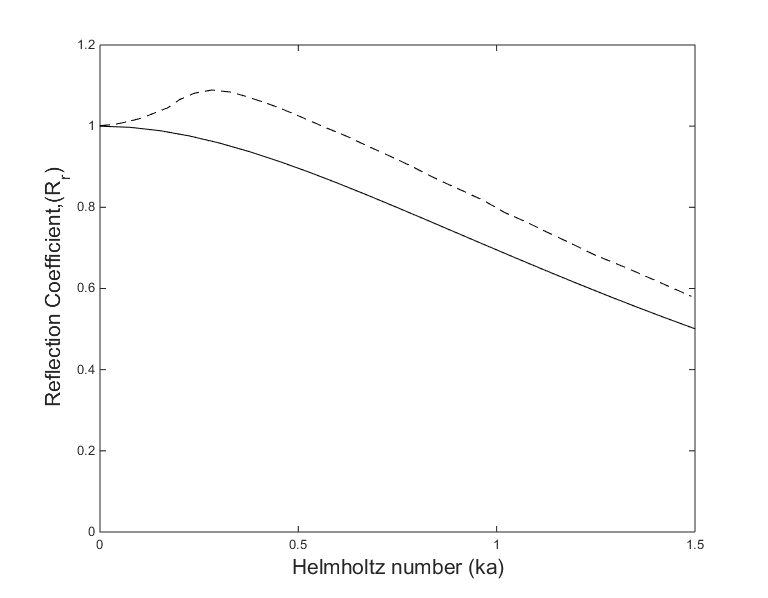
\includegraphics[width=.9\linewidth]{figuras/abs_r_comparacao.png}
  \caption[Magnitudes do coeficiente de reflexão $|R|$]{Resultados analíticos exatos para magnitude do coeficiente de reflexão $\|R\|$ ao final de um duto não flangeado. A linha contínua apresenta o resultado sem escoamento de \citeonline{levine1948radiation} e a linha tracejada apresenta o resultado com escoamento de Mach = 0,15 de \citeonline{munt1990acoustic}.}
  \label{fig:comp1}
\end{figure}

Como é mostrado na Figura \ref{fig:comp1}, a magnitude do coeficiente de reflexão $\|R\|$ aumenta consideravelmente na presença de um escoamento subsônico. Além disso, pode-se perceber que, em algumas frequências, $\|R\|$ torna-se maior do que a unidade, implicando que a amplitude da onda refletida torna-se maior do que a da onda incidente. Este fenômeno ocorre, sobretudo, pela transferência de energia cinética rotacional do escoamento para o campo acústico. Essa transferência de energia cinética ocorre sobretudo pelo desprendimento periódico de vórtices na borda do duto.

\begin{figure}[ht!]
\centering
  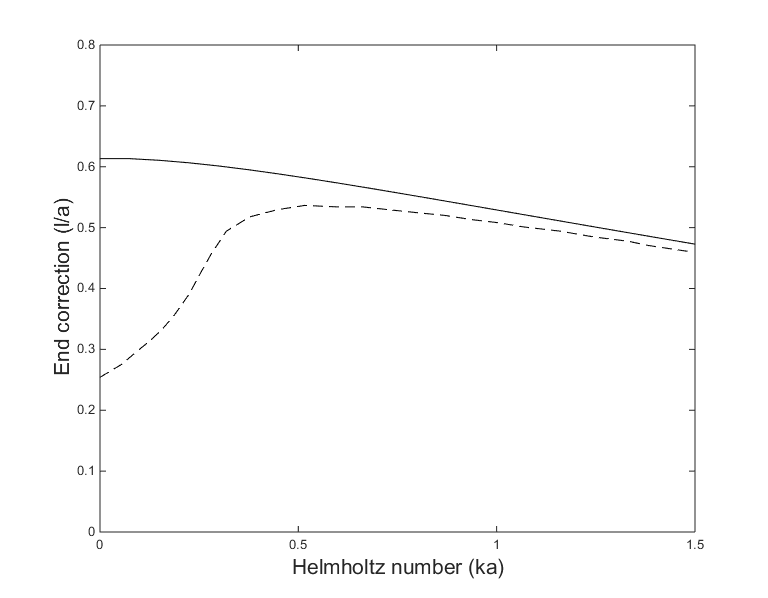
\includegraphics[width=.9\linewidth]{figuras/loa_comparacao.png}
  \caption[Coeficientes de correção de terminação $l/a$]{Resultados analíticos exatos para o coeficiente de correção da terminação normalizado pelo raio $l/a$ de um duto não flangeado. A linha contínua apresenta o resultado sem escoamento de \citeonline{levine1948radiation} e a linha tracejada apresenta o resultado com escoamento de Mach = 0,15 de \citeonline{munt1990acoustic}.}
  \label{fig:comp2}
\end{figure}
\newpage
De acordo com a Figura \ref{fig:comp2}, a correção normalizada da terminação $l/a$ torna-se consideravelmente menor do que aquela obtida na ausência de escoamento, sobretudo para baixos números de helmholtz ($ka$)\simbolo{$ka$}{Número de helmholtz}. Em outras palavras, para baixas frequências e na presença de um escoamento a onda acústica é refletida em uma região mais próxima da abertura, em comparação à situação sem escoamento.

No que diz respeito a modelos analíticos aproximados, o trabalho de \citeonline{carrier1955sound} foi um dos primeiros a abordar o cálculo do coeficiente de reflexão e correção da terminação com escoamento de exaustão num duto não flangeado. Para tal foi considerado um gás perfeito invíscido com o tipo de escoamento uniforme (\textit{plug}). Nessa abordagem usou-se a mesma metodologia que \citeonline{levine1948radiation} porém acoplando à formulação matemática o método de Prandtl-Glauert.

\citeonline{mani1973refraction} deu prosseguimento a mesma abordagem de \citeonline{carrier1955sound} com escoamento de exaustão, porém considerando a continuidade do deslocamento das partículas acústicas transversais. Esse tipo de solução mostra diversos fenômenos antes não previstos com os outros modelos citados como efeitos de convecção, zonas de silêncio relativo e refrações.

Também na mesma linha de desenvolvimento de \citeonline{carrier1955sound}, \citeonline{savkar1975radiation} desenvolveu um modelo de modos de alta ordem com escoamento de exaustão e sucção do tipo \textit{plug} com variação de temperatura. A continuidade do deslocamento das partículas acústicas transversais também foi considerada, possibilitando assim análises de fenômenos de convectivos.

\citeonline{rienstra1980} também desenvolveu um modelo matemático aproximado para o cálculo dos coeficientes de reflexão e terminação do duto não flangeado. A contribuição desse trabalho foi a inclusão dos parâmetros do meio externo ao duto como velocidade do som, densidade e velocidade de escoamento. Com esse modelo foi possível investigar como o meio externo influencia na acústica interna do duto e as limitações da condição de Kutta.

Em relação a trabalhos experimentais, \citeonline{ingard1975} investigaram o coeficiente de reflexão em dutos quadrados em regime de escoamento succionado de Mach 0,4. O método de medição se baseou na técnica de dois microfones e os mesmos foram ajustados para números de helmholtz ($ka$) menores que 0,5. Em vista desse contexto experimental, o autor desenvolveu uma fórmula analítica para o cálculo do coeficiente de reflexão.

Na mesma linha de investigação, \citeonline{davies1987} investigou o coeficiente de reflexão porém com dutos circulares não flangeados e flangeados. O autor destaca que a disposição geométrica da terminação do duto, quando submetida a fenômenos de escoamentos succionados, desenvolve a chamada \textit{vena} contracta, que pode ser estimada e associada com o fator de perda $Kp$\simbolo{$Kp$}{Fator de perda}. Em vista dos procedimentos desse trabalho, o autor compara os resultados com o estudo de \citeonline{ingard1975} e sugere um aperfeiçoamento na equação analítica do cálculo do coeficiente de reflexão.

No que diz respeito a escoamentos de exaustão o trabalho de \citeonline{allam2006investigation} abordou um sistema super determinado de medição para investigação da acústica interna de um duto não flangeado. Para contornar a dificuldade de medição do coeficiente de correção da terminação do duto, surgiu-se como motivação o desenvolvimento de um sistema em que há mais microfones do que incógnitas a serem calculadas, em outras palavras, extendeu-se a metodologia de medição de 2 microfones para mais que 4 microfones. Há de se considerar também que a parte imaginária do número de onda, parte associada com a dissipação de energia por viscosidade, não pode ser obtida quando há escoamento e por isso foi incluída como incógnita. Em linhas gerais esse trabalho permitiu a validação experimental do trabalho de \citeonline{munt1990acoustic} e a consolidação de um sistema confiável de medição para esse tipo de problema.

\citeonline{english2010} investigou também de forma experimental os coeficientes de reflexão e de terminação de dutos circulares com diferentes espessuras. Focando para números de Mach entre 0 e 0,3, seus resultados mostram que os coeficientes de reflexão estão com valores acima dos que são encontrados no trabalho de \citeonline{munt1990acoustic}. O autor explica esse fato relatando que a condição de Kutta subestima o surgimento de vórtices na saída do duto.




\chapter{Metodologia}

Tal como foi discutido no capítulo anterior, para a investigação do coeficiente de reflexão na presença de escoamento, faz-se ncessária a utilização de esquemas numéricos que integrem na mesma estrutura a parte fluido dinâmica e acústica. Neste sentido, o método de lattice Boltzmann mostra-se adequado, sobretudo quando são considerados baixos números de Mach ($M$ $<$ 0,2) e baixos números de Reynolds ($Re$ $<$ 5515). Nesse sentido, há traballhos que validam, aplicam e desenvolvem metodologias de \textit{lattice} Boltzmann no campo de estudo da aeroacústica.

Um desses estudos é o de \citeonline{crouse2006fundamental}, que mostraram a eficácia do método de \textit{lattice} Boltzmann em recuperar as equações de Navier-Stokes para baixas compressibilidades ($M$ $<$ 0,3). Há de se ressaltar que validaram também o modelo numérico de um ressonador de Helmholtz com um modelo experimental do mesmo, demonstrando assim a viabilidade da aplicação para problemas de acústica.

No que se trata de desenvolvimento de ferramentas auxiliares para tratar problemas acústicos, \citeonline{kam2006non} desenvolveram uma condição de contorno absorvente, baseada na técnica de camadas perfeitamente casadas (``\textit{perfectly} \textit{matched} \textit{layers}''). Essencialmente, a técnica se baseia na criação de uma camada com viscosidade crescente exponencialmente na direção exterior do domínio computacional.

\citeonline{marie2009} analisou e comparou esquemas de alta ordem das equações de Navier-Stokes linearizadas com o método de \textit{lattice} Boltzmann. O objeto de estudo para comparação foi análises de dispersão e dissipação de ondas acústicas em regime isotérmico. Conclui-se com esse trabalho que para um erro de dispersão pré-definido, o método de \textit{lattice} Boltzmann se comportou como mais rápido.

No que diz respeito a aplicação do método de \textit{lattice} Boltzmann num problema de aeroacústica, \citeonline{lew2010noise} desenvolveram um modelo numérico em 3D para predição de ruído em um jato turbulento subsônico. Como validação, os resultados foram comparados com resultados experimentais e cálculos numéricos feitos a base de \textit{Large} \textit{Eddy} \textit{Simulation} (LES)\abreviatura{LES}{\textit{Large} \textit{Eddy} \textit{Simulation}}. Esse estudo demonstrou as principais vantagens de se trabalhar com o método de \textit{lattice} Boltzmann como por exemplo o baixo custo computacional e a facilidade em inserir \textit{nozzles} com formas complexas no domínio computacional.

Também na área de aeroacústica computacional, o trabalho de \citeonline{shi2013lattice} propõe um modelo em \textit{lattice} Boltzmann para obter dados de diretividade da radiação sonora num duto circular submetido a escoamento subsônico. Os resultados de diretividade foram comparados com os modelos de \citeonline{levine1948radiation} e \citeonline{gabard2006}, mostrando uma boa convergência principalmente nas baixas frequências.

Já no sentido de tratamento de fenômenos da acústica básica, \citeonline{viggen2013acoustic} adicionou termos fonte na equação de \textit{lattice} Boltzmann para que o método possa permitir o surgimento de dipolos, quadrupolos e outras superposições de multipolos. Além disso, esses termos foram mapeados nos parâmetros macroscópicos através da ferramenta matemática de expansão de Chapman-Enskog. Como resultado, conseguiu reproduzir fenômenos de diretivade de monopolos, dipolos e quadrupolos.

\citeonline{da2015assessment} abordaram também o uso do método de \textit{lattice} Boltzmann em conjunto com a técnica de \textit{Large} \textit{Eddy} \textit{Simulation} (LES) na investigação do ruído gerado na interação do escoamento de um jato com uma placa plana. Os dados de níveis de pressão sonora em campo distante foram obtidos usando uma superfície de Ffowcs-Williams e Hawkings (FW-H)\abreviatura{FW-H}{Superfície de Ffowcs-Williams e Hawkings} e comparados com dados experimentais.

O presente Capítulo apresenta o método de lattice Boltzmann utilizado neste trabalho e descreve a construção de um modelo tridimensional de duto não-flangeado utilizando a plataforma de código aberto Palabos. Detalhes sobre a elaboração do modelo são discutidos detalhadamente nas seções subsequentes.

\section{O Método de Lattice Boltzmann}

O método de \textit{lattice} Boltzmann possui bastante utilidade quando se trata de problemas aeroacústicos, envolvendo pequenas flutuações de pressão e fenômentos de turbulência. Isso se deve ao fato do método ter surgido de uma outra abordagem de fenômenos mecânicos aplicados a fluidos - uma abordagem microscópica de interações entre moléculas.

Uma solução para resolver problemas fluidodinâmicos através de interações entre moléculas é abordar o fenômeno físico pelo ponto de vista de distribuição de moléculas, a qual se convêm chamar de partícula. Nesse caso, cada partícula é descrita a partir de uma função de distribuição, a qual indica a probabilidade de se encontrar numa dada região espacial e em um determinado instante de tempo, um conjunto de moléculas que compartilham a mesma velocidade e direção de propagação. A equação de transporte que rege a propagação das partículas e a difusão da quantidade de movimento das mesmas a partir de suas colisões é a Equação de Boltzmann que, ao ser discretizada, pode ser resolvida numericamente originando assim o método de \textit{lattice} Boltzmann ou \textit{lattice} \textit{Boltzmann} \textit{Method} (LBM)\abreviatura{LBM}{\textit{Lattice} \textit{Boltzmann} \textit{Method}}. 

Historicamente o método de \textit{lattice} Boltzmann se originou nos anos 90 através de trabalhos como de \citeonline{he1997theory}, que mostraram que a forma discreta da equação de Boltzmann também recupera as equações de Navier Stokes para baixas compressibilidades (baixos números de Mach). Isto fornece uma ligação formal entre as equações macroscópicas de lattice Boltzmann e as equações de Navier-Stokes para baixas compressibilidades, além de possibilitar a implementação computacional desse método.

O LBM possui muitas vantagens em relação a técnicas tradicionais de fluido dinâmica computacional aplicadas a aeroacústica: resolve o campo acústico e o campo fluido dinâmico numa mesma iteração em cada incremento de tempo, extração direta do campo de pressão e fácil implementação paralela elevando assim a performance frente a outros métodos.

\subsection{Modelo BGK}

O LBM é baseado em operações de colisão e propagação de funções de distribuição de partículas com massa em função do tempo e espaço. Cada conjunto de funções de distribuição localizadas num ponto no espaço $\textbf{x}$ e tempo $t$ pode ser chamada de célula e, segundo o trabalho de \citeonline{he}, a equação de \textit{lattice} Boltzmann, que formula o comportamento de cada célula, pode ser escrita como 
\begin{equation}
	f_{i}(\textbf{x} + c_{i}\Delta t, t + \Delta t) = f_{i}(\textbf{x}, t) + \Omega_{i}(f(\textbf{x}, t)),
    \label{eq:f_i}
\end{equation}
sendo $i$ é um número inteiro que delimita direções no espaço de propagação de partículas, $f_{i}$ é a função de distribuição em uma dada direção $i$, $c_{i}$ são velocidades de propagação na direção $i$ e $\Delta t$ é o incremento de tempo. 
\simbolo{$f_{i}$}{Função de distribuição LBM na direção $i$}
\simbolo{$i$}{Direção de propagação LBM}
\simbolo{$c_{i}$}{Velocidades de propagação na direção $i$}
\simbolo{$\textbf{x}$}{Localização espacial de uma célula LBM}
\simbolo{$t$}{Localização temporal de uma célula LBM}
\simbolo{$\Delta t$}{Incremento discreto de tempo}

A Equação (\ref{eq:f_i}) é dividida nas duas operações básicas: propagação e colisão. O lado esquerdo dessa equação representa a operação de propagação, na qual os valores das funções de distribuição de cada célula são movidos para cada direção de propagação para uma próxima célula no espaço em cada iteração no tempo. Feita a operação de propagação, é realizada a operação de colisão, representada pelo lado direito da equação, na qual o termo $\Omega_{i}$\simbolo{$\Omega_{i}$}{Operador de colisão LBM} representa o operador de colisão.

Uma das formas de calcular o operador de colisão $\Omega_{i}$ é usar a formulação proposta no estudo de \citeonline{bgk}. A aplicação dessa formulação consolida o modelo BGK (Bhatnagar–Gross–Krook)\abreviatura{BGK}{Bhatnagar–Gross–Krook} ou modelo de tempo de relaxação único: \textit{single}-\textit{relaxation}-\textit{time} (SRT)\abreviatura{SRT}{\textit{single}-\textit{relaxation}-\textit{time}}. Nesse sentido, o operador de colisão é definido por
\begin{equation}
	\Omega_{i} = -\frac{1}{\tau}(f_{i} - f_{i}^{M}),
    \label{eq:omega_i}
\end{equation}
tal que $\tau$\simbolo{$\tau$}{Período de colisão LBM} é o período de colisão, período médio de colisão entre partículas, e $f_{i}^{M}$\simbolo{$f_{i}^{M}$}{Função de distribuição de Maxwell ou de equilíbrio} é a função de distribuição de Maxwell ou função de distribuição de equilíbrio.

A função de distribuição de Maxwell $f_{i}^{M}$ pode ser calculada aplicando o princípio de máxima entropia de acordo com as retrições das leis de conservação de massa e quantidade de movimento, assim como é proposto por \citeonline{wolf}. Dessa forma a função de distribuição de Maxwell é definida por
\begin{equation}
	f_{i}^{M} = \rho \varepsilon _{i}\bigg( 1 + \frac{\textbf{u}.c_{i}}{c_{s}^{2}} + \frac{\textbf{u}.c_{i}^{2} - c_{s}^{2}\textbf{u}}{2c_{s}^{4}}\bigg),
    \label{eq:f_i_M}
\end{equation}
sendo que $\rho$ é a densidade local do fluido, $\varepsilon_{i}$ são pesos de velocidades para cada direção de propagação $i$, $\textbf{u}$ é a velocidade local do fluido, $c_{i}$ é um vetor de velocidades de propagação da célula para cada direção $i$ e $c_{s}$ é a velocidade do som.
\simbolo{$\rho$}{Densidade local do fluido}
\simbolo{$\varepsilon_{i}$}{Pesos de velocidades para cada direção de propagação $i$}
\simbolo{$\textbf{u}$}{Velocidade local do fluido}
\simbolo{$c_{s}$}{Velocidade do som}

Os parâmetros macroscópicos de densidade local do fluido $\rho$ e a velocidade local do fluido $\textbf{u}$ podem ser obtidos a partir dos momentos da função de distribuição $f_{i}$ das seguintes maneiras

\begin{equation}
  \rho = \sum{f_{i}} \text{   e }
    \label{eq:rho}
\end{equation}
\begin{equation}
  \rho \textbf{u} = \sum{f_{i} c_{i}}.
    \label{eq:u}
\end{equation}

A partir da equação de estado isoentrópica linear, a pressão local do fluido $p$ pode ser obtida na forma
\begin{equation}
  p = \rho c^{2}_{s}.
    \label{eq:p}
\end{equation}

A viscosidade cinemática $\nu$ é um parâmetro que é função do período de colisão $\tau$ e pode ser obtida com a equação
\begin{equation}
	\nu = c^{2}_{s} \bigg(\tau - \frac{1}{2}\bigg).
    \label{eq:nu}
\end{equation}
\simbolo{$p$}{Pressão local do fluido}
\simbolo{$\nu$}{Viscosidade cinemática do fluido}

Quando as equações \ref{eq:rho}, \ref{eq:u}, \ref{eq:p} e \ref{eq:nu} são usadas para recuperar os atributos macroscópicos do fluido a unidade de medida não é uma unidade física. Segudo o trabalho de \citeonline{da2016prediction}, para se ter esses atributos em unidade física é preciso aplicar regras de conversão. Essas regras de conversão se baseiam em duas constantes que são definidas a partir de unidades físicas: velocidade característica definida por   
\begin{equation}
  \zeta = c^{*}/c_{s},
    \label{eq:conversao_1}
\end{equation}
em que $c^{*}$ é a velocidade física do som, e discretização $\Delta x$ definida pelo tamanho de uma célula dado em metros.

Com os parâmetros $c^{*}$ e $\Delta x$ pode-se realizar as seguintes conversões para unidades físicas, notadas com o superíndice $*$:

\begin{equation}
  \textbf{$u^{*}$} = \zeta \textbf{$u$}\text{, }
  \label{eq:conversao_2}
\end{equation}

\begin{equation}
  \textbf{$x^{*}$} = \Delta x\textbf{$x$}\text{, }
  \label{eq:conversao_3}
\end{equation}
  
\begin{equation}
  t^{*} = \frac{\Delta x}{\zeta}t \text{, }
  \label{eq:conversao_4}
\end{equation}

\begin{equation}
  \nu^{*} = \zeta \Delta x \nu\text{, }
  \label{eq:conversao_5}
\end{equation}

\begin{equation}
  \rho^{*} = \frac{\zeta}{\Delta x} \rho \text{, }
  \label{eq:conversao_6}
\end{equation}

\begin{equation}
  p^{*} = p \zeta^{2}  \rho^{*}_{0} \text{ e }
  \label{eq:conversao_7}
\end{equation}

\begin{equation}
  f^{*} = f\frac{\zeta}{\Delta x},
  \label{eq:conversao_8}
\end{equation}

tal que $f^{*}$ e $f$ são unidades de frequências física e do LBM respectivamente\simbolo{$f^{*}$}{Frequência física}\simbolo{$f$}{Frequência em LBM}.

Há várias geometrias de células, o grupo do tipo $D_{n}Q_{b}$ ($n$ dimensões e $b$ direções de propagação ou velocidades) é um dos mais usados e foi proposto por \citeonline{qian1992lattice}. A tabela \ref{table:modelos} mostra os parâmetros para cada um dos modelos do tipo $D_{n}Q_{b}$, seus diferentes vetores de velocidades de propagação ($c_{i}$), seus respectivos pesos $\varepsilon_{i}$ e as suas constantes de velocidade do som ($c_{s}$). Esses valores são obtidos para cada geometria, de forma que se mantenham a conservação da massa e da quantidade de movimento. Portanto com esses parâmetros já se torna possível calcular a função de Maxwell ($f_{i}^{M}$) para cada operação de colisão em cada iteração de tempo.

Para esse trabalho usou-se o modelo D3Q19 e a Figura \ref{fig:d3q19} ilustra um esquemático desse tipo de célula e é possível visualizar espacialmente as direções de propagação. Vale ressaltar que para cada direção há o cáculo da função de Maxwell ($f_{i}^{M}$) e, por conseguinte, a operação de propagação das funções de distribuição para a célula adjacente no sentido de cada direção.

\begin{table}[ht!]
\centering
\caption{Modelos $D_{n}Q_{b}$}
\label{table:modelos}
\begin{tabular}{|c|c|c|c|}
\hline
Modelo & $c_{i}$ & $\varepsilon_{i}$ & $c_{s}^{2}$ \\ \hline
%-----------------------------------------------------------------------------
D1Q3   & $0$,                        & $2/3$,                   & $1/3$ \\
   	   & $\pm 1$                     & $1/6$                    &     \\ \hline
%-----------------------------------------------------------------------------
   	   & $0$,                        & $6/12$,				    &  \\
D1Q5   & $\pm 1$,                    & $2/12$,			        & $1$ \\  
       & $\pm 2$                     & $1/12$			        &    \\ \hline
%-----------------------------------------------------------------------------
D2Q7   & $(0,0)$,                  & $1/2$,                    & $1/4$ \\ 
	   & $(\pm 1/2, \pm \sqrt{3}/2)$ & $1/12$                  &    \\ \hline
%-----------------------------------------------------------------------------
       & $(0,0)$,                     & $4/9$,                    &    \\
D2Q9   & $(\pm 1,0)$, $(0,\pm 1)$,    & $1/9$,                    & $1/3$   \\
   	   & $(\pm 1,\pm 1)$              & $1/36$                    &    \\ \hline
%-----------------------------------------------------------------------------
	   & $(0,0,0)$,                           & $2/9$,            &   \\ 
D3Q15  & $(\pm 1,0,0)$, $(0,\pm 1,0)$, $(0,0,\pm 1)$, & $1/9$,   & $1/3$ \\ 
	   & $(\pm 1, \pm 1,\pm 1)$               & $1/72$           &   \\ \hline
%-----------------------------------------------------------------------------
	   & $(0,0,0)$,                           & $1/3$,                        &    \\ 
D3Q19  & $(\pm 1,0,0)$, $(0,\pm 1,0)$, $(0,0,\pm 1)$, & $1/18$,               & $1/3$ \\ 
	   & $(\pm 1,\pm 1,0)$, $(\pm 1,0,\pm 1)$, $(0,\pm 1,\pm 1)$ & $1/36$,    &    \\ \hline 
\end{tabular}
\end{table}

\begin{figure}[ht!]
\centering
  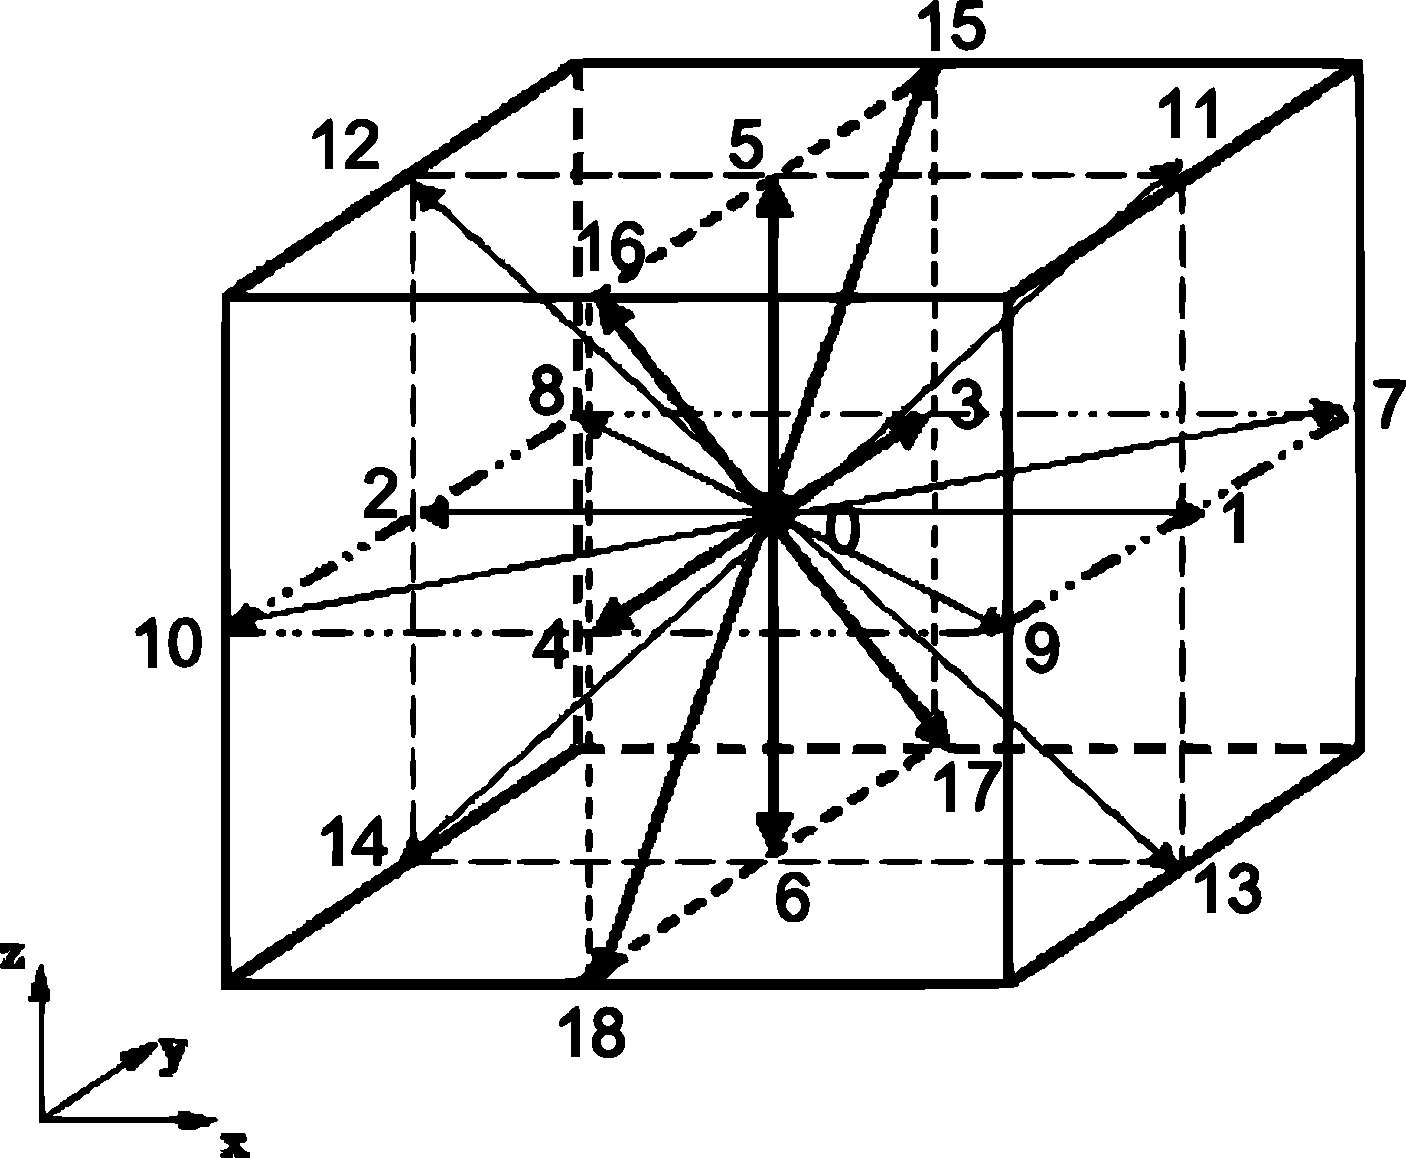
\includegraphics[width=.75\linewidth]{figuras/d3q19.pdf}
  \caption[Esquemático do D3Q19]{Esquemático do modelo D3Q19. Ilustração adaptada do estudo de \citeonline{premnath2013investigation}.}
  \label{fig:d3q19}
\end{figure}

\newpage
\subsection{Múltiplos Tempos de Relaxação}

A Equação (\ref{eq:omega_i}) retrata um operador de colisão com tempo de relaxação único para todas as direções de propagação $i$. Essa abordagem é funcional, porém limitada à estabilidade em baixos números de Reynolds como mostra o estudo de \citeonline{lallemand2000theory}. Para esses tipos de problemas a abordagem de múltiplos tempos de relaxação (MRT)\abreviatura{MRT}{\textit{multiple}-\textit{relaxation}-\textit{time}}, pode ser usada assim como é mostrado nos estudos de \citeonline{viggen2014lattice}.

Seguindo a formulação proposta por \citeonline{d1994generalized}, a formulação de MRT se baseia na troca do parâmetro de único tempo de relaxação $\tau$ por uma matriz \textbf{$\Lambda$} de vários tempos de relaxação. Todavia a matriz \textbf{$\Lambda$} é construída de acordo com uma matriz \textbf{$M$} que projeta as funções de distribuição $f_{i}$ e $f_{i}^{M}$ no espaço dos momentos. De acordo com \citeonline{lallemand2000theory}, a possibilidade desse método ser mais estável é oriunda da capacidade de operar a colisão das células com um tempo de relaxação apropriado para cada um dos vários momentos, projetados a partir das funções de distribuição $f_{i}$ e $f_{i}^{M}$. Em vista do exposto o operador de colisão da Equação (\ref{eq:omega_i}) se transforma em
\begin{equation}
	\Omega_{i} = -\textbf{$\Lambda$}(f_{i} - f_{i}^{M}).
    \label{eq:MRT_1}
\end{equation}
Porém a operação de colisão é realizada no espaço dos momentos. Logo é preciso projetar $f_{i}$ e $f_{i}^{M}$ no espaço dos momentos impondo
\begin{equation}
	m_{i} = \textbf{$M$}f_{i} \text{ e } m_{i}^{M} = \textbf{$M$}f_{i}^{M}.
    \label{eq:MRT_2}
\end{equation}
\citeonline{d1994generalized} propôs, para o caso do modelo D3Q19, uma distribuição de valores para a matriz \textbf{$M$} dada por

% \begin{equation}
%   \tiny {\begin{bmatrix}
% a & b & t \\
% \end{bmatrix}  }
% \end{equation}

\setcounter{MaxMatrixCols}{19}
\begin{equation}
\textbf{$M$} = 
\tiny{\begin{bmatrix}
A &   A &   A &   A &   A &   A &   A &   A &   A &   A &   A &   A &   A &   A &   A &   A &   A &   A &   A \\ 
 B & C & C & C & C & C & C &   D &   D &   D &   D &   D &   D &   D &   D &   D &   D &   D &   D \\ 
  E &  F &  F &  F &  F &  F &  F &   A &   A &   A &   A &   A &   A &   A &   A &   A &   A &   A &   A \\ 
   G &   A &  J &   G &   G &   G &   G &   G &   G &   G &   G &  J &   A &  J &   A &  J &   A &  J &   A \\ 
   G &  F &   K &   G &   G &   G &   G &   G &   G &   G &   G &  J &   A &  J &   A &  J &   A &  J &   A \\ 
   G &   G &   G &   A &  J &   G &   G &   A &  J &  J &   A &   G &   G &   G &   G &   A &  J &  J &   A \\ 
   G &   G &   G &  F &   K &   G &   G &   A &  J &  J &   A &   G &   G &   G &   G &   A &  J &  J &   A \\ 
   G &   G &   G &   G &   G &   A &  J &   A &  J &   A &  J &  J &   A &   A &  J &   G &   G &   G &   G \\ 
   G &   G &   G &   G &   G &  F &   K &   A &  J &   A &  J &  J &   A &   A &  J &   G &   G &   G &   G \\ 
   G &   I &   I &  J &  J &  J &  J &  H &  H &  H &  H &   A &   A &   A &   A &   A &   A &   A &   A \\ 
   G &  F &  F &   I &   I &   I &   I &  H &  H &  H &  H &   A &   A &   A &   A &   A &   A &   A &   A \\ 
   G &   G &   G &   A &   A &  J &  J &   G &   G &   G &   G &  J &  J &  J &  J &   A &   A &   A &   A \\ 
   G &   G &   G &  H &  H &   I &   I &   G &   G &   G &   G &  J &  J &  J &  J &   A &   A &   A &   A \\ 
   G &   G &   G &   G &   G &   G &   G &   G &   G &   G &   G &   G &   G &   G &   G &  J &  J &   A &   A \\ 
   G &   G &   G &   G &   G &   G &   G &   A &   A &  J &  J &   G &   G &   G &   G &   G &   G &   G &   G \\ 
   G &   G &   G &   G &   G &   G &   G &   G &   G &   G &   G &   A &   A &  J &  J &   G &   G &   G &   G \\ 
   G &   G &   G &   G &   G &   G &   G &   G &   G &   G &   G &   A &  J &   A &  J &  J &   A &  J &   A \\ 
   G &   G &   G &   G &   G &   G &   G &   A &  J &  J &   A &   G &   G &   G &   G &  J &   A &   A &  J \\ 
   G &   G &   G &   G &   G &   G &   G &  J &   A &  J &   A &  J &   A &   A &  J &   G &   G &   G &   G \\
\end{bmatrix}},
\end{equation}
sendo $A = 1$, $B = -30$, $C = -11$, $D = 8$, $E = 12$, $F = -4$, $G = 0$, $H = -2$ e $I = 2$.

Considerando que a matriz \textbf{$S$} é dada por
\begin{equation}
	\textbf{$S$} = \textbf{$M$}\textbf{$\Lambda$}\textbf{$M$}^{-1},
    \label{eq:MRT_3}
\end{equation}
o operador de colisão fica
\begin{equation}
	\Omega_{i} = -\textbf{$M$}^{-1}\textbf{$S$}(m_{i} - m_{i}^{M}).
    \label{eq:MRT_4}
\end{equation}
Inserindo a Equação (\ref{eq:MRT_4}) na Equação (\ref{eq:f_i}) fica
\begin{equation}
	f_{i}(\textbf{x} + c_{i}\Delta t, t + \Delta t) = f_{i}(\textbf{x}, t) -\textbf{$M$}^{-1}\textbf{$S$}(m_{i} - m_{i}^{M}).
    \label{eq:MRT_5}
\end{equation}
Vale ressaltar que a operação de propagação, lado esquerdo da Equação (\ref{eq:MRT_5}), ocorre no espaço original da função de distribuição $f_{i}$.


\subsection{Condições de Contorno}

\subsubsection{\textit{Bounceback}}

De acordo com o estudo de \citeonline{viggen2014lattice}, a condição de contorno do tipo \textit{bounceback} tem como objetivo simular uma parede rígida no domínio do LBM, sendo ela do tipo implícita e localizada entre as células. Há dois tipos de \textit{bounceback}: \textit{free-slip}, que simula escorregamento livre do fluido na parede e \textit{no-slip}, que impõe que todas as componentes de velocidade junto à parede sejam nulas. Essa condição força o desenvolvimento da camada limite viscosa junto à parede. Nesse trabalho foi usado a condição do tipo \textit{no-slip}, afim de capturar os efeitos de camada limite viscosa.

A condição de contorno \textit{bounceback} \textit{no-slip} é geralmente implementada na etapa de propagação a partir de uma inversão de funções de distribuição de partículas. A Figura \ref{fig:bounceback} mostra um esquemático de exemplo do processo de funcionamento dessa condição de contorno. Ao cruzar a condição de contorno no tempo seguinte $t + \Delta t$, a célula inverte as funções de distribuição de partículas para o sentido contrário dos vetores que apontam para o \textit{bounceback}.

% \begin{figure}[ht!]
% \centering
%   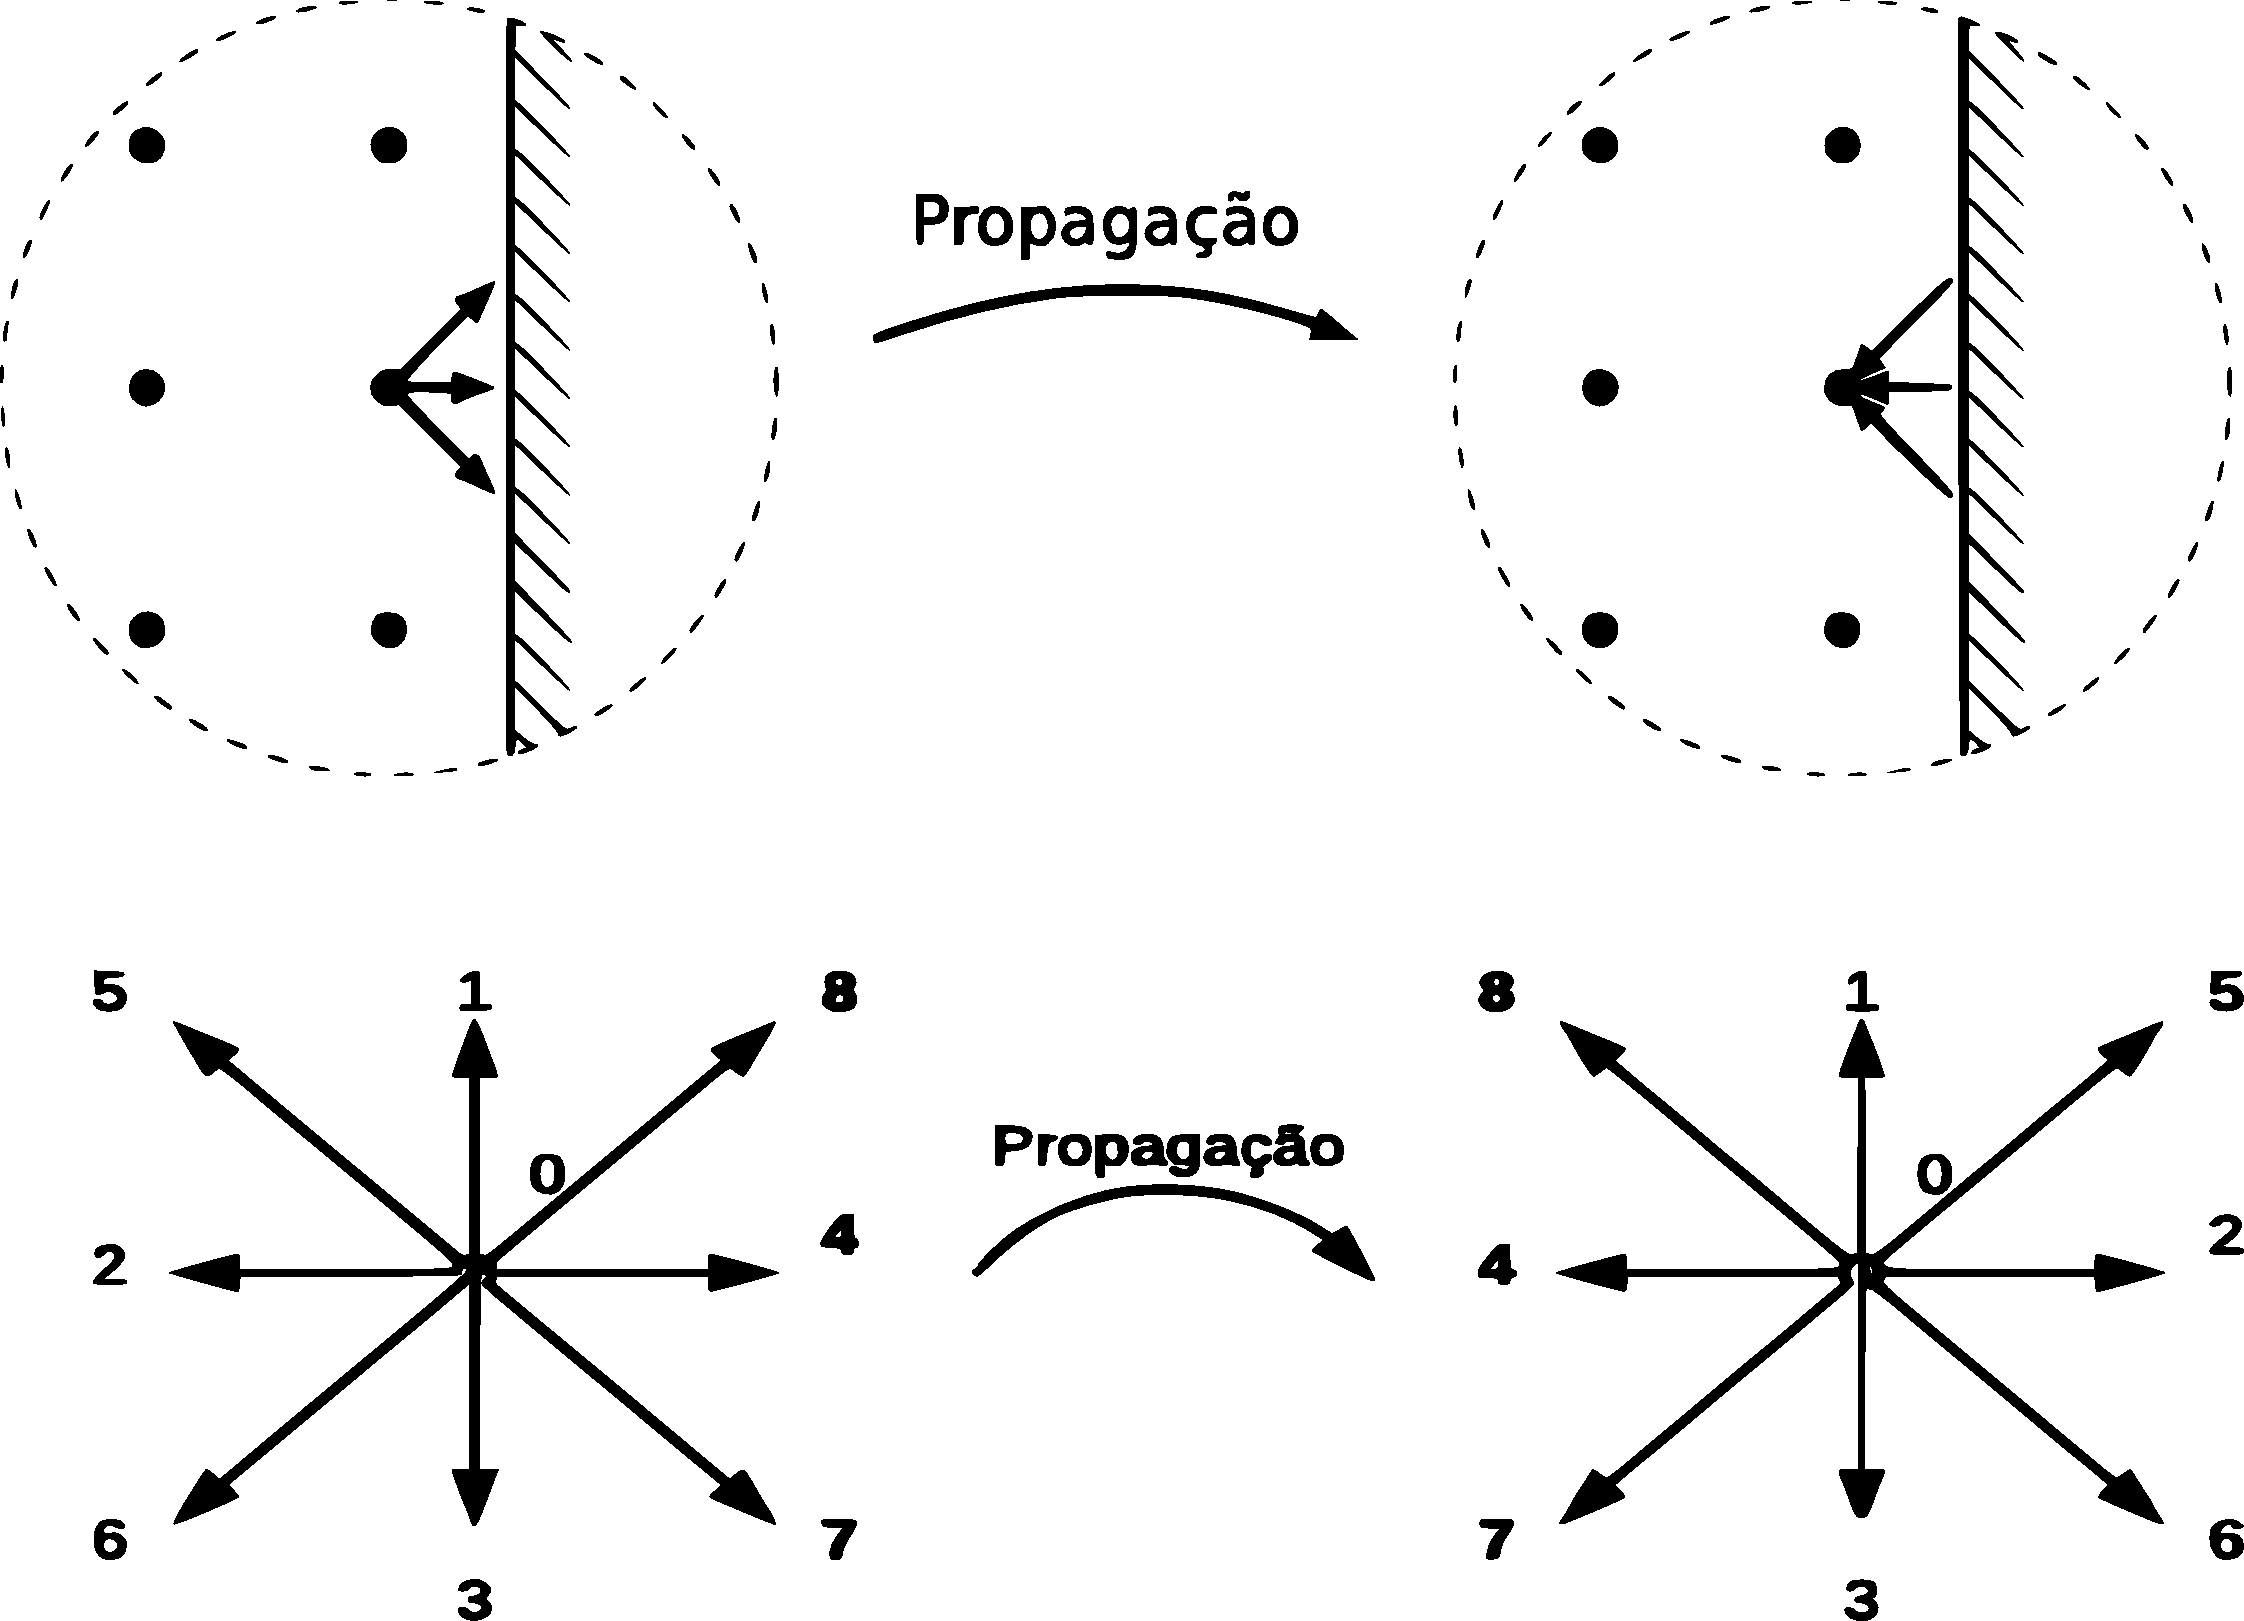
\includegraphics[width=.65\linewidth]{figuras/bounceback.pdf}
  
%   \label{fig:bounceback}
% \end{figure}

\begin{figure}[ht!]
  \centering
  \def\svgwidth{200pt}
  \import{figuras/}{bounceback_2.pdf_tex}
  \caption[Funcionamento do \textit{bounceback} \textit{no-slip}]{Esquemático de exemplo do processo de funcionamento da condição de contorno \textit{bounceback} \textit{no-slip}. Ilustração adaptada do estudo de \citeonline{viggen2014lattice}.}
  \label{fig:bounceback}
\end{figure}

\newpage
Em relação às equações de propagação o processo abordado fica

\begin{gather*}
  f_{6}(\textbf{x}, t + \Delta t) = f_{8}(\textbf{x}, t)\text{,  } f_{8}(\textbf{x}, t + \Delta t) = f_{6}(\textbf{x}, t), \\
  f_{2}(\textbf{x}, t + \Delta t) = f_{4}(\textbf{x}, t)\text{,  } f_{4}(\textbf{x}, t + \Delta t) = f_{2}(\textbf{x}, t) \text{, }\\
  f_{5}(\textbf{x}, t + \Delta t) = f_{7}(\textbf{x}, t)\text{ e } f_{7}(\textbf{x}, t + \Delta t) = f_{5}(\textbf{x}, t).
\label{eq:bounceback}
\end{gather*}

\subsubsection{Condição Anecóica}

Consolidar uma condição do tipo anecóica num método numérico de natureza temporal é um desafio em todos os métodos numéricos. Nesse contexto, considerando a absorção de ondas de pressão, entropia e pulsos de despredimento de vórtices, o trabalho de \citeonline{kam2006non} propõe uma condição de contorno explícita de absorção. Em essência, este método se baseia na adaptação do método das camadas perfeitamente casadas (``\textit{perfectly} \textit{matched} \textit{layers}") para o LBM. A condição de contorno de absorção, \textit{Absorbing} \textit{Boundary} \textit{Condition} (ABC)\abreviatura{ABC}{\textit{Absorbing} \textit{Boundary} \textit{Condition}}, consiste na adição de uma região de amortecimento para que os valores de pressão e velocidade convirjam assintoticamente a valores que caracterizam um fluido em repouso. Nesse sentido, valores alvos para um fluido em resposo de densidade ($\rho_{T}$ $=$ $\rho_{0}$) e velocidade (\textbf{$u_{T}$} $=$ $0$) são usados para calcular uma função de distribuição de amortecimento $f_{i}^{T}$\simbolo{$f_{i}^{T}$}{Função de distribuição de amortecimento}. Essa função de distribuição é definida da mesma forma que $f_{i}^{M}$, porém com os valores alvos de densidade e velocidade, impostos na forma
\begin{equation}
  f_{i}^{T} = \rho_{0}\varepsilon_{i}.
  \label{eq:f_alvo}
\end{equation}
Como essa técnica é explícita, o operador de colisão $\Omega_{i}$ da Equação (\ref{eq:omega_i}) é adaptado e recebe um novo termo fonte, tal que
\begin{equation}
  \Omega_{i} = -\frac{1}{\tau}(f_{i} - f_{i}^{M}) - \sigma(f_{i}^{M} - f_{i}^{T}),
  \label{eq:omega_i_abc}
\end{equation}
sendo $\sigma$ $=$ $\sigma_{T}(\delta/D)^{2}$ o coeficiente de absorção, $\sigma_{T}$ uma constante com valor de $0,3$, $\delta$ é a distância medida do começo da região de contorno no sentido da convergência assintótica e $D$ é o tamanho total da região de contorno no sentido da convergência assintótica assim como ilustra a Figura \ref{fig:abc}.

\begin{figure}[ht!]
\centering
  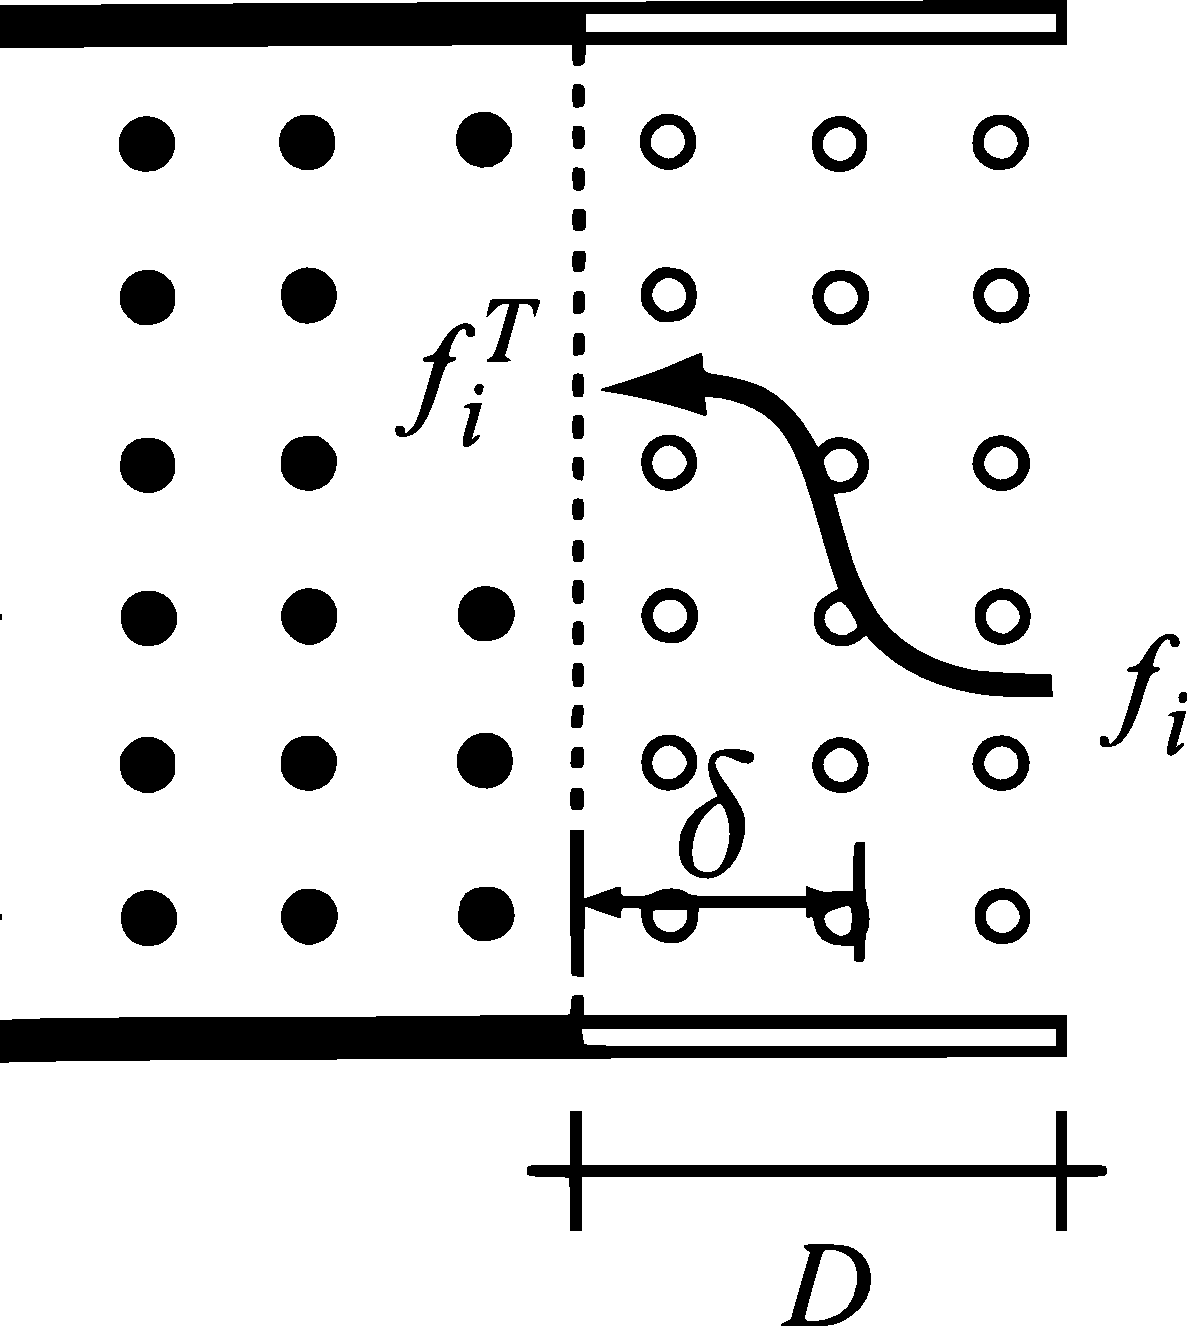
\includegraphics[width=.3\linewidth]{figuras/abc.pdf}
  \caption[Funcionamento da condição de contorno anecóica]{Esquemático de exemplo do processo de funcionamento da condição de contorno anecóica. Ilustração adaptada do estudo de \citeonline{da2008numerical}.}
  \label{fig:abc}
\end{figure}

O operador de colisão da Equação (\ref{eq:omega_i_abc}) funciona bem para o modelo SRT, porém como nesse estudo será usado o modelo MRT, algumas adaptações precisam ser realizadas, pois a operação de colisão ocorre no espaço dos momentos nesse modelo. Assim como é feito nas Equações (\ref{eq:MRT_2}) deve-se aplicar o mesmo procedimento na função de distribuição $f_{i}^{T}$ originando o termo $m_{i}^{T}$. Além disso é preciso inserir esse termo no operador de colisão da Equação (\ref{eq:MRT_4}) resultando em 

\begin{equation}
  \Omega_{i} = -\textbf{$M$}^{-1}\textbf{$S$}(m_{i} - m_{i}^{M}) - 
  \sigma\textbf{$M$}^{-1}\textbf{$S$}(m_{i}^{M} - m_{i}^{T}).
  \label{eq:abc_mrt_2}
\end{equation}

Simplificando, a Equação (\ref{eq:abc_mrt_2}) fica
\begin{equation}
  \Omega_{i} = -\textbf{$M$}^{-1}\textbf{$S$}[m_{i} - m_{i}^{M}(\sigma - 1) - m_{i}^{T}].
  \label{eq:abc_mrt_3}
\end{equation}

Adicionando esse termo na Equação geral (\ref{eq:f_i}) do LBM, o resultado é a equação
\begin{equation}
  f_{i}(\textbf{x} + c_{i}\Delta t, t + \Delta t) = f_{i}(\textbf{x}, t) -\textbf{$M$}^{-1}\textbf{$S$}[m_{i} - m_{i}^{M}(\sigma - 1) - m_{i}^{T}].
  \label{eq:abc_mrt_4}  
\end{equation}

A Equação (\ref{eq:abc_mrt_4}) equivale a Equação (\ref{eq:f_i}) porém com um termo fonte adicional representando a camada anecóica. Vale ressaltar que esse termo fonte é nulo no domínio fluidodinamico e diferente de zero na camada absorvente.

\section{Palabos}

O \textit{software} livre Palabos é um projeto feito na linguagem C++ no paradígma computacional de orientação a objetos, resultado da colaboração entre indústria e academia, focando produzir uma ferramenta de simulação computacional robusta, rápida e confiável. Junto com esse pacote computacional há implementados modelos numéricos de publicações e \textit{benchmarks} da litetura, como mostra os estudos de \citeonline{lattice_1}, \citeonline{lattice_2}, \citeonline{lattice_3}, \citeonline{lattice_4} e \citeonline{lattice_5}. 

As funcionalidades do \textit{software} Palabos usadas nesse trabalho são: modelo base (MRT); condição de contorno (\textit{bounceback} \textit{no-slip}); \textit{grid} (D3Q19); paralelismo (MPI em vários processadores); dados de saída (ASCII, GIF e VTK para visualização no \textit{software} \citeonline{paraview}).

Mesmo com várias funcionalidades citadas, o \textit{software} Palabos precisa ter outras outras funcionalidades implementadas para que possa atender o escopo desse trabalho. Para atender esse requisito, o projeto \citeonline{palabos_acoustic} foi criado como uma versão do Palabos que contém todos os modelos e implementações desenvolvidas nesse trabalho. As funcionalidades desenvolvidas nesse trabalho são: condição de contorno anecóica de \citeonline{kam2006non} para BGK D2Q9 e MRT D2Q9 e D3Q19; condição de contorno para excitação do duto com \textit{sweep} de acordo com o estudo de \citeonline{da2009sound} ou excitação por soma de harmônicos.


\section{Modelo Numérico}

Com os arquivos de compilação e execução corretamente configurados, pode-se modelar numericamente o problema. A Figura \ref{fig:modelo} representa a vista do corte lateral do modelo numérico tridimensional com o eixo de coordenadas localizado no ponto $(\frac{\textbf{Nx}}{2}, 0, 0)$. Para a definição do domínio foi utilizado uma abordagem paramétrica, ou seja, o raio externo do duto $a$ $=$ $20$ células foi a unidade de medida para as dimensões. As dimensões \textbf{Nx} e \textbf{Ny} são iguais e possuem $20a$ de comprimento (razão de aspecto não mantida no esquema para economia do espaço em folha). A dimensão \textbf{Nz} possui 79,5$a$ de comprimento e foi baseado no estudo de \citeonline{da2009sound}, que justifica a distância da saída do duto até a parede para capturar corretamente os efeitos de inércia e elasticidade produzidos pelo fluido estagnante ao redor do duto. Todo espaço de fluido do domínio foi preenchido em cada célula com frequência de relaxação $\frac{1}{\tau}$ $=$ $1,99$, $\rho$ $=$ $\rho_{0}$ $=$ $1$ e as velocidades para todos os sentidos $u_{x}$ $=$ $u_{y}$ $=$ $u_{z}$ $=$ $0$. As bordas do duto foram preenchidas com condição anecóica de espessura igual 1,5$a$ células.      

Com relação ao duto, o mesmo possui o tamanho \textbf{L} $=$ $18a$ e é delimitado pela condição de contorno \textit{bounceback} \textit{no-slip}. O diâmetro externo mede $2a$ e parede com expessura de 0,1$a$. No começo do duto há uma condição anecóica com espessura igual a 1,5$a$, que é responsável pela absorção da onda refletida na abertura do duto. Ao lado da condição anecóica há uma condição de contorno de excitação do duto com espessura de 0,05$a$, responsável por excitar os modos axiais e impor escoamento.    

% \begin{figure}[ht!]
%   \centering
%   \def\svgwidth{400pt}
%   \import{figuras/}{modelo_numerico.pdf_tex}
%   \caption[Esquemático do modelo numérico]{Esquemático do modelo numérico: vista do corte lateral do modelo em 3D.}
%   \label{fig:modelo}
% \end{figure}

\begin{figure}[ht!]
\centering
  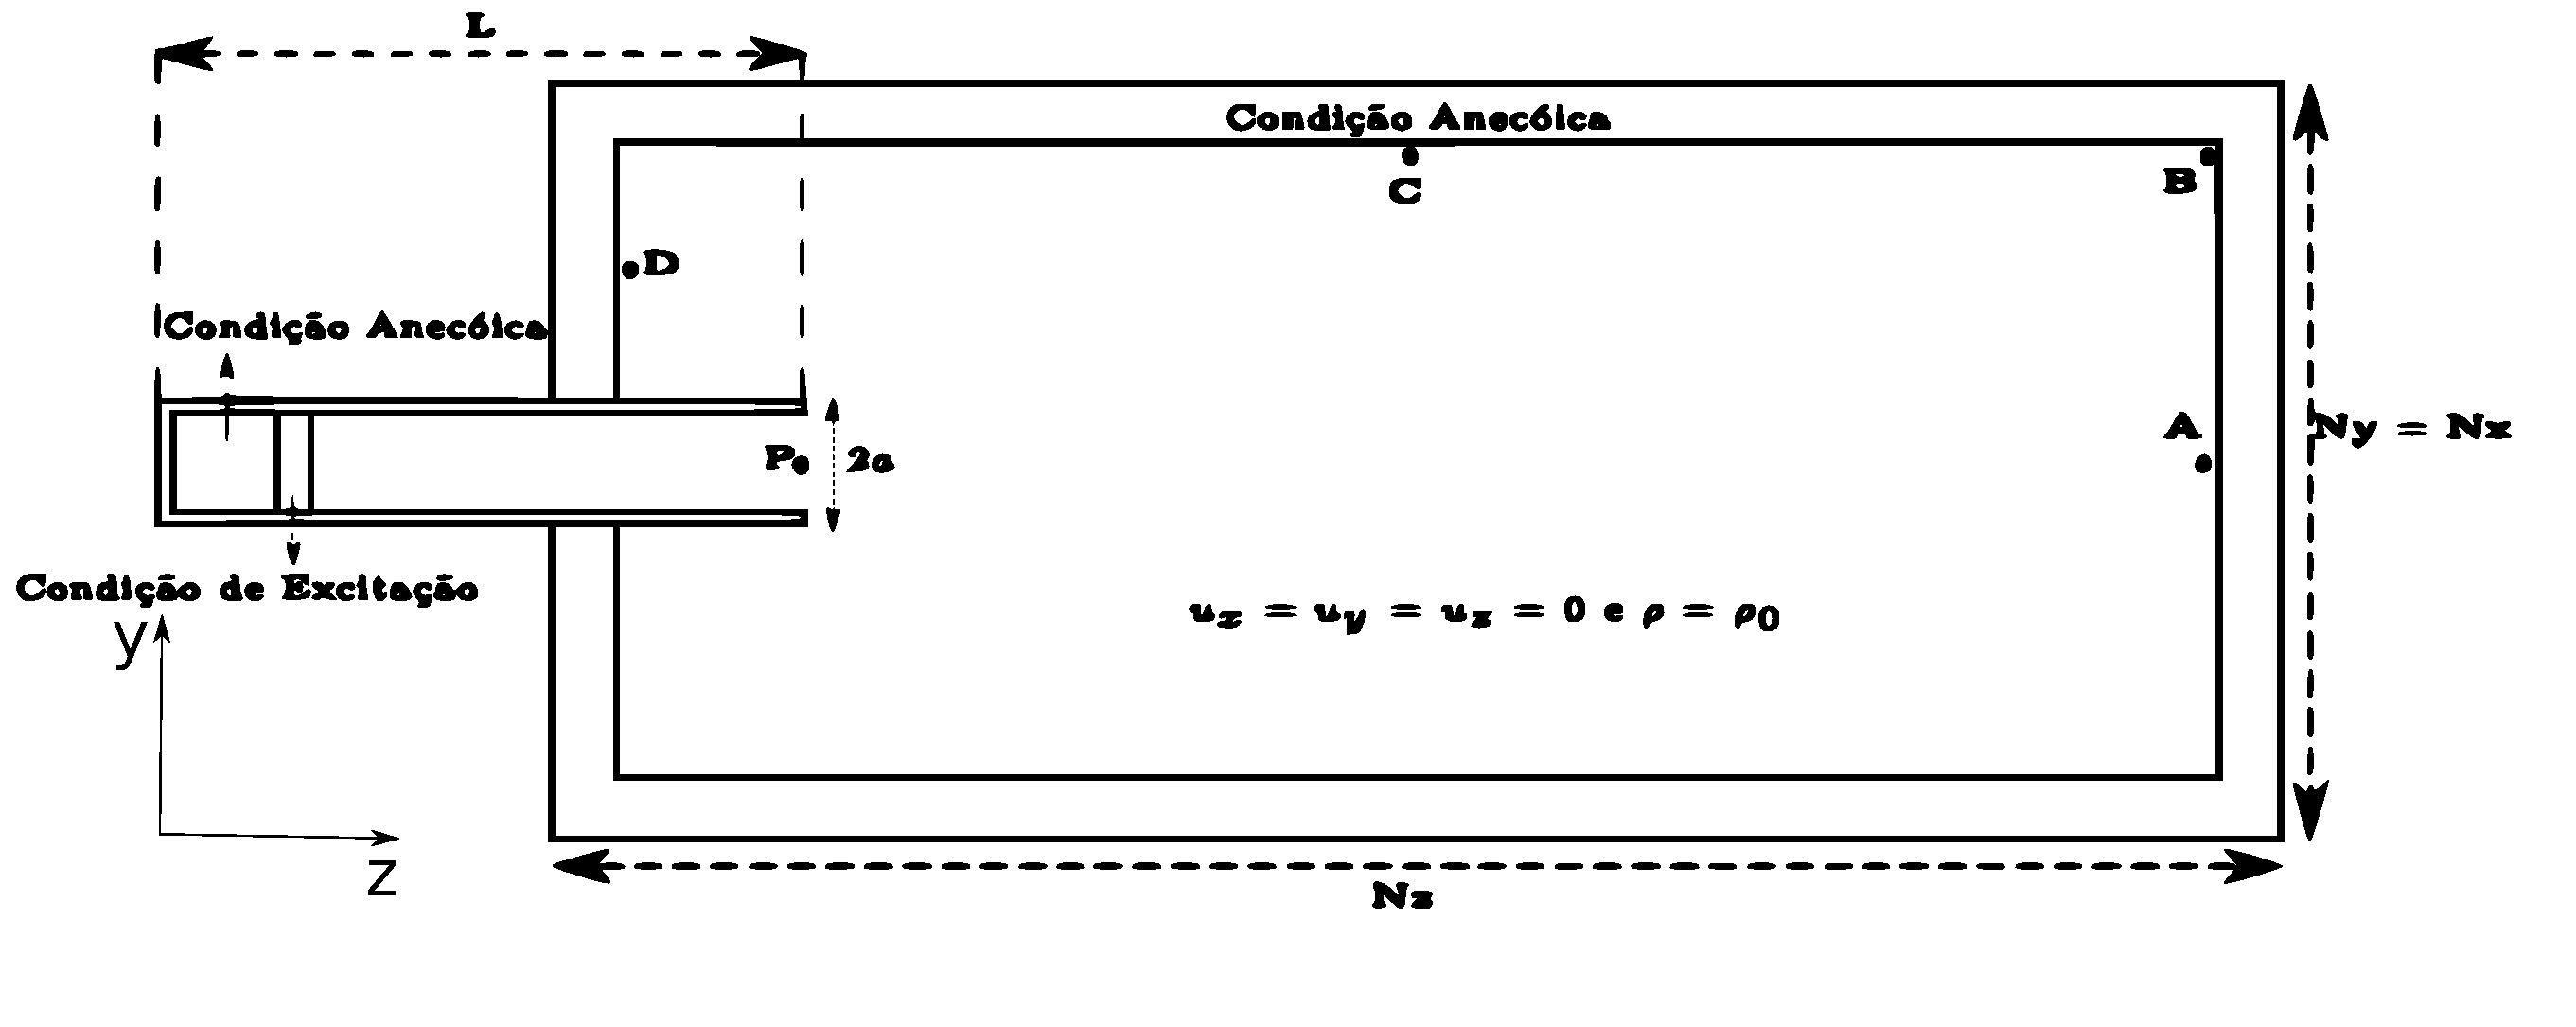
\includegraphics[width=1.\linewidth]{figuras/modelo_numerico_3.pdf}
  \caption[Esquemático do modelo numérico]{Esquemático do modelo numérico: vista do corte lateral do modelo em 3D.}
  \label{fig:modelo}
\end{figure}


Focando propiciar energia suficiente nos modos axiais com onda plana, a condição de excitação foi desenvolvida através de uma soma de ondas estacionárias, na faixa de frequência $0$ $<$ $ka$ $\leq$ 2,5. Dessa forma, os valores de densidade e velocidade dessa região foram mudados em cada incremento de tempo da seguinte forma:
\begin{itemize}
  \item regime transiente ($0 \leq t < t_{transiente}$):
  \begin{gather*}
    \rho(t) = \rho_{0};% + A\sum_{n=1}^{N} sin\bigg(\frac{nka_{max}c_{s}t}{Na}\bigg);
    \\ u_{z}(t) = Mc_{s};    
    \\ u_{y}(t) = 0;
    \\ u_{x}(t) = 0.
  \label{eq:transiente}
  \end{gather*}

  \item regime estacionário ($t_{transiente} \leq t \leq t_{total} - t_{propagada}$):
  \begin{gather*}
    \rho(t) = \rho_{0} + A\sum_{n=1}^{N} sin\bigg(\frac{nka_{max}c_{s}t}{Na}\bigg);
    \\ u_{z}(t) = Mc_{s} + \frac{Ac_{s}}{\rho_{0}}\sum_{n=1}^{N} sin\bigg(\frac{nka_{max}c_{s}t}{Na}\bigg);    
    \\ u_{y}(t) = 0;
    \\ u_{x}(t) = 0.
  \label{eq:estacionario}
  \end{gather*}
\end{itemize}
tal que $ka_{max} =$ 2,5, $N$ é o número total de componentes harmônicos dentro do intervalo $0$ $<$ $ka$ $\leq$ 2,5, $n$ é a $n$-ésima componente harmônica dentro desse intervalo. $t_{transiente}$ é é o número de incrementos de tempo necessessários para atingir o regime estacionário. Este valor se baseou no estudo de \citeonline{shi2013lattice} na forma $t_{transiente} =  2\textbf{Nz}/Mc_{s}$, $t_{propagada}$ é definido como $t_{propagada} = \textbf{Nz}/c_{s}$ e é o tempo que a onda demora para percorrer o domínio completo na direção axial do duto, $t_{total} = t_{transiente} + t_{propagada} + 12000$ é o tempo total da simulação e $A$ é definida em termos de densidade. Esta é calculada por
\begin{equation}
  A = \frac{2 \cdot 10^{-5} \cdot 10^{\text{NPS}/20}}{c^{*}\rho^{*}_{0}c_{s}},
\end{equation}
tal que $c^{*} = 343$ $m/s$ é a velocidade do som em unidades físicas, $\rho^{*}_{0} =$ 1,22 $kg/m^{3}$ é a densidade física do ar em unidades físicas e NPS é o nível de pressão sonora no valor de 80 dB.

\subsection{Verificação da Condição Anecóica}

No intuito de avaliar a condição anecóica nas fronteiras do domínio através do cálculo e análise do coeficiente de reflexão, os pontos $\textbf{A}$, $\textbf{B}$, $\textbf{C}$ e $\textbf{D}$ representados na Figura \ref{fig:modelo} são utilizados para medição de pressão e velocidade de partícula acústica na fronteira com a terminação anecóica. O local dos pontos é definido pelas seguintes coordenadas:

\begin{itemize}
  \item ponto $\textbf{A}$: $(\frac{\textbf{Nx}}{2}, \frac{\textbf{Ny}}{2}, \textbf{Nz} - 31)$;
  \item ponto $\textbf{B}$: $(\frac{\textbf{Nx}}{2}, \textbf{Ny} - 31, \textbf{Nz} - 31)$;
  \item ponto $\textbf{C}$: $(\frac{\textbf{Nx}}{2}, \textbf{Ny} - 31, \frac{\textbf{Nz}}{2})$;
   \item ponto $\textbf{D}$: $(\frac{\textbf{Nx}}{2}, \frac{3\textbf{Ny}}{4}, 12a + 31)$.
\end{itemize}
 
Já o ponto $\textbf{P}$ representa a média espacial, feita no plano transversal do duto, dos valores de pressão e velocidade de partícula na terminação. Essas médias espaciais são extraídas e calculadas ao longo do tempo para se obter os parâmetros de caracterização da acústica interna do duto: coeficiente de reflexão $R_{r}$ e coeficiente de correção da terminação $l/a$.

Para a execução da simulação numérica foi escolhido um \textit{hardware} com as seguintes características:

\begin{itemize}
  \item arquitetura: x86\_64;
  \item CPU(s): 8;
  \item modelo do processador: Intel(R) Xeon(R) CPU E5620 @2.40GHz;
  \item memória RAM: 139 GB.
\end{itemize}

%\newcommand{\MyNumberA}{30}

%\newcommand{\MyNumberB}{60}

%\MyNumberB

%\numexpr (\MyNumberA + 2* \MyNumberN)/3 \relax
%\the\numexpr (\MyNumberA * \MyNumberB)

\section{Pós-processamento}

Com os arquivos de dados temporais dos pontos $\textbf{A}$, $\textbf{B}$, $\textbf{C}$, $\textbf{D}$ e da média espacial $\textbf{P}$ salvos em disco rígido, um \textit{script} de pós-processamento da plataforma \citeonline{matlab}/\citeonline{octave} é executado. Os seguintes procedimentos são realizados no \textit{script}:

\begin{enumerate}
  \item os vetores temporais de pressão e velocidade no eixo axial são obtidos através da leitura de arquivos \textbf{.dat};
  \item uma janela Hanning na forma
  \begin{equation}
    w(n) = sin^{2}\bigg(\frac{\pi n}{N - 1} \bigg),  
  \end{equation}
  tal que $N$ é o tamanho da janela e $n$ é a posição do vetor unidimensional é definida e usada para multiplar os sinais de velocidade e pressão no domínio do tempo;

  \item a transformada discreta de Fourier, utilizando o algorítmo de transformada rápida, \textit{Fast} \textit{Fourier} \textit{Transform} (FFT)\abreviatura{FFT}{\textit{Fast} \textit{Fourier} \textit{Transform}}, foi utilizada para transformar os históricos temporais de pressão e velocidade de partícula para o domínio da frequência;

  \item a impedância de radiação $Z_{r}$ é calculada através da divisão entre os vetores de pressões por de velocidades no domínio da frequência da seguinte forma:
  \begin{equation}
    Z_{r} = \frac{p(f)}{u_{z}(f)};
  \end{equation}

  \item a magnitude do coeficiente de reflexão $|R_{r}|$ é calculado de acordo com a Equação (\ref{eq:R});
  \item o coeficiente de correção da terminação $l/a$ é calculado de acordo com a Equação (\ref{eq:l});
 \end{enumerate}

 Para minimizar os efeitos não lineares de ondas evanescentes na terminação do duto e o efeito da espessura do duto (equivalente a duas células), um fator de correção $c = - 0,2367$ é adicionado na parte real do coeficiente de correção da terminação $l/a$.

Para fins de comparação dos resultados obtidos nesse estudo com resultados da literatura foi usado o coeficiente de correlação de Pearson na forma
\begin{equation}
  r = \Bigg|\frac{\sum_{j=1}^{J} (x_{j} - \overline{x})(y_{j} - \overline{y})}{\sqrt{\sum_{j=1}^{J} (x_{j} - \overline{x})^{2}} \sqrt{\sum_{j=1}^{J} (y_{j} - \overline{y})^{2}}}\Bigg| \times 100,
\end{equation}
tal que $r$ é um percentual, sendo que quanto maior o valor mais correlacionado o resultado do modelo numérico estará com modelos da literatura. $J$ é o número total de pontos, $x_{j}$ e $y_{j}$ são valores de dois conjuntos de pontos na posição $j$ a serem comparados e $\overline{x}$ e $\overline{y}$ são as médias definidas nas formas
\begin{equation}
  \overline{x} = \frac{\sum_{j=1}^{J} x_{j}}{J} \text{ e }
\end{equation}
\begin{equation}
  \overline{y} = \frac{\sum_{j=1}^{J} y_{j}}{J}. 
\end{equation}

\section{Colorário de Howe}

Em vista da literatura vigente, fenômenos aeroacústicos envolvendo baixos números de Reynolds são muito peculiares pelo fato do campo acústico ser alterado pela transferência de energia cinética vorticial em energia acústica e vice-versa. Para investigar tal fenomenologia, o corolário de energia de Howe apresenta-se como uma ferramenta apelativa.

De acordo com o estudo de \citeonline{howe1984absorption} o colorário é uma descrição formal da transferência da energia cinética vorticial para o campo acústico e vice-versa num contexto de baixos números de Mach ($M << 1$) e escoamentos isoentrópicos. Tal formulação é expressa por 

\begin{equation}
  <P> = -\rho_{0}\int_{V}< \boldsymbol{\xi} > dV,
\end{equation}
tal que $<P>$\simbolo{$<P>$}{Potência acústica} é a potência acústica média ao longo de um ciclo de oscilação em torno de um volume $V$, $\rho_{0}$ é a densidade média do fluido e $\boldsymbol{\xi}$\simbolo{$\boldsymbol{\xi}$}{Energia acústica} é a energia acústica instantânea por unidade de volume gerada a partir da energia cinética vorticial. A energia acústica é expressa por 
\begin{equation}
  \boldsymbol{\xi} = \textbf{u}_{ac} \cdot ( \boldsymbol{\omega} \times \textbf{u}),
\end{equation}
tal que $\textbf{u}_{ac}$\simbolo{$\textbf{u}_{ac}$}{Velocidade de partícula} é a velocidade de partícula, $\boldsymbol{\omega}$\simbolo{$\boldsymbol{\omega}$}{Rotacional do escoamento} é o rotacional do escoamento e $\textbf{u}$ é a velocidade do escoamento. Para o uso do colorário de Howe, foi implementada uma classe dentro do núcleo do \textit{software} Palabos, sendo ativada e instanciada no final de cada simulação do modelo numérico.     
\chapter{Resultados}

Em vista da teoria vigente na literatura e pelo que foi exposto no ponto de vista metodológico, obteve-se resultados nos seguintes contextos:
\begin{itemize}
  \item análise da condição anecóica: a partir dos históricos temporais de pressão e velocidade de partícula nas fronteiras do modelo numérico, foram feitas análises críticas de reflexão acústica;
  \item duto sem escoamento: a partir dos históricos temporais de pressão e velocidade de partícula na terminação do duto, foram feitas validações e análises críticas dos parâmetros caracterizadores da acústica interna do duto sem escoamento;
  \item duto com escoamento de exaustão: a partir dos históricos temporais de pressão e velocidade de partícula na terminação do duto, foram feitas validações e análises críticas dos parâmetros caracterizadores da acústica interna do duto com escoamento de exaustão para regimes subsônicos ($M$ $\leq$ 0,2);
  \item duto com escoamento sugado: a partir dos históricos temporais de pressão e velocidade de partícula na terminação do duto, foram feitas validações, análises críticas e investigação dos parâmetros caracterizadores da acústica interna do duto com escoamento succionado para regimes subsônicos ($M$ $\leq$ 0,2).
\end{itemize} 

\section{Análise da Condição Anecóica}

Com a finalidade de mensurar e analisar o comportamento da condição de contorno anecóica por meio de métricas numéricas e objetivas, foram calculados impedâncias e coeficientes de reflexão nas fronteiras do modelo numérico, ou seja, nos pontos \textbf{A}, \textbf{B}, \textbf{C} e \textbf{D} como é mostrado na Figura \ref{fig:modelo}. As Figuras \ref{fig:resultados_A}, \ref{fig:resultados_B}, \ref{fig:resultados_C} e \ref{fig:resultados_D} mostram os resultados nos respectivos pontos citados.


% \begin{figure}
% \begin{center}
% \begin{tikzpicture}
% \begin{axis}[
%     title={},
%     width=0.9\textwidth,
%     height=0.45\textwidth,
%     xlabel={Frequência},
%     ylabel={Sensibilidade},
%     x unit={\space Hz \space},
% 	y unit={\space C/g \space},
%     ytick=data,
%     xmin=0,
%     ymin=0,
%     ymax=0.55,
%     legend pos=north west,
%     grid=minor, % Display a grid	
% 	grid style={dashed,gray!90}, % Set the style
% 	]
%      %\addplot[color=black,dashed,thick,mark=*,mark options={solid},smooth] table[x index=2,y index=3] {Data/Kollias_SBMR_095_exp.txt}; \label{Kollias_exp095}
%      %\addlegendentry{Experimental (Kollias)}
%       %\addplot[color=blue,semithick] table[x index=0,y index=1] {Data/Kollias_SBMR_095_exp.txt}; \label{Kollias_sim095}
%     %\addlegendentry{Simulação (Kollias)}
%              \addplot[color=black, thick] table[x index=0,y index=1] {dados/coeficiente_reflexao_anecoica/A_real.txt};
%              \addplot[color=black,dashed,  thick] table[x index=0,y index=1] {dados/coeficiente_reflexao_anecoica/A_imag.txt};
%               \label{Comsol_095}% \addlegendentry{Simulação (Comsol)}
% \end{axis}
% \end{tikzpicture}
%  \caption{Resposta em carga do acelerômetro para $r$ igual a 0,95.}
% \end{center}
% \end{figure}

\newcommand\scalexA{0.8}
\newcommand\scaleyA{0.8}
\newcommand\scalex{1}
\newcommand\scaley{1}
\newcommand\scaleA{0.5}

\newpage

A Figura \ref{fig:resultados_A} mostra os resultados de parâmetros de caracterização de reflexão no ponto \textbf{A}, ou seja, num ponto que está a frente da terminação do duto. Pode-se observar pela Figura \ref{fig:A_impedancia} que a parte real da impedância converge para o valor de $\rho_{0} c_{0}$ de referência na literatura, que em unidades do LBM possui o valor igual 0,57735. A parte imaginária da Figura \ref{fig:A_impedancia} converge num valor bem abaixo, porém ainda distante de 0 como é o ideal de uma situação totalmente anecóica. A Figura \ref{fig:A_reflexao} confirma o fato que se vê na Figura \ref{fig:A_impedancia}, ou seja, vê-se a mesma tendência do coeficiente de reflexão na parte imaginária do gráfico de impedância, ocasionando aproxidamente 15\% de reflexão. Vale ressaltar também da Figura \ref{fig:A_reflexao} que para baixas frequências há uma alta reflexão. 

\begin{figure}[ht!]
\begin{subfigure}{\scaleA \textwidth}
  % impedancia A
\begin{tikzpicture}
\begin{axis}[
width=\scalex \textwidth,
height=\scaley \textwidth,
xmin=0,
xmax=2.5,
ymin=0,
ymax=0.55,
ytick distance=0.1,
xtick distance=0.5,
grid=major, % Display a grid  
%grid style={dashed,gray!90}, % Set the style
xlabel = \small{$ka$},
ylabel = \small{$Z_{\textbf{A}}$},
]
\addplot[color=black, thick] table[x index=0,y index=1] {dados/coeficiente_reflexao_anecoica/A_real.txt};
\addplot[color=black,dashed,  thick] table[x index=0,y index=1] {dados/coeficiente_reflexao_anecoica/A_imag.txt};

\end{axis}
\end{tikzpicture}
\caption[Impedância $Z_{\textbf{A}}$]{}
\label{fig:A_impedancia}
%\caption[Impedância $Z_{\textbf{A}}$]{Resultado da impedância calculada no ponto $\textbf{A}$, próximo da condição anecóica localizada nas fronteiras do modelo numérico. A linha contínua representa a parte real e a linha tracejada representa a parte imaginária.}
\end{subfigure}%
\begin{subfigure}{\scaleA \textwidth}
  % reflexao A
\begin{tikzpicture}
\begin{axis}[
width=\scalex \textwidth,
height=\scaley \textwidth,
xmin=0,
xmax=2.5,
ymin=0,
ymax=1,
ytick distance=0.2,
xtick distance=0.5,
grid=major, % Display a grid  
%grid style={dashed,gray!90}, % Set the style
xlabel = \small{$ka$},
ylabel = \small{$|R_{\textbf{A}}|$},
]
\addplot[color=black, thick] table[x index=0,y index=1] {dados/coeficiente_reflexao_anecoica/A_abs.txt};

\end{axis}
\end{tikzpicture}
%\caption[Coeficiente de Reflexão $R_{\textbf{A}}$]{Resultado da magnitude do coeficiente de reflexão calculado no ponto $\textbf{A}$, próximo da condição anecóica localizada nas fronteiras do modelo numérico.}
\caption[Coeficiente de Reflexão $R_{\textbf{A}}$]{}
\label{fig:A_reflexao}
\end{subfigure}
\caption[Resultados de reflexão no ponto \textbf{A}]{Resultados da impedância $Z_{\textbf{A}}$ (\ref{fig:A_impedancia}) e módulo do coeficiente de reflexão $|R_{\textbf{A}}|$ (\ref{fig:A_reflexao}) calculados no ponto $\textbf{A}$. Na Figura (\ref{fig:A_impedancia}) a linha contínua representa a parte real e a linha tracejada representa a parte imaginária.}
\label{fig:resultados_A}
\end{figure}

A Figura \ref{fig:resultados_B} mostra os resultados de parâmetros de caracterização de reflexão no ponto \textbf{B}, ou seja, numa região de descontinuidade na direção $z$ e $y$. Pode-se observar pela Figura \ref{fig:B_impedancia} que a parte real e imaginária da impedância diverge consideravelmente de uma condição anecóica ideal. Tal fato pode ser verificado na Figura \ref{fig:B_reflexao} que, embora o coeficiente de reflexão não convirja para 1, há a presença de reflexões principalmente em baixas frequências. Mesmo o ponto \textbf{B} tendo uma tendência distoante de uma condição anecóica ideal, considera-se tal fato como desprezível visto que há poucas regiões descontínuas dessa condição de contorno no modelo numérico. 

\begin{figure}
\begin{subfigure}{\scaleA \textwidth}
  \begin{tikzpicture}
  \begin{axis}[
	width=\scalex \textwidth,
  height=\scaley \textwidth,
	xmin=0,
  xmax=2.5,
    ymin=0,
    ymax=0.9,
    ytick distance=0.2,
    xtick distance=0.5,
    grid=major, % Display a grid	
 	%grid style={dashed,gray!90}, % Set the style
	xlabel = \small{Número de Helmholtz ($ka$)},
	ylabel = \small{Impedância ($Z_{\textbf{B}}$)},
  ]
 \addplot[color=black, thick] table[x index=0,y index=1] {dados/coeficiente_reflexao_anecoica/B_real.txt};
   \addplot[color=black,dashed,  thick] table[x index=0,y index=1] {dados/coeficiente_reflexao_anecoica/B_imag.txt};
   
  \end{axis}
  \end{tikzpicture}
  \caption[Impedância $Z_{\textbf{B}}$]{}
  \label{fig:B_impedancia}
  %\caption[Impedância $Z_{\textbf{B}}$]{Resultado da impedância calculada no ponto $\textbf{B}$, próximo da condição anecóica localizada nas fronteiras do modelo numérico. A linha contínua representa a parte real e a linha tracejada representa a parte imaginária.}
  
\end{subfigure}%
\begin{subfigure}{\scaleA \textwidth}
  \begin{tikzpicture}
  \begin{axis}[
	width=\scalex \textwidth,
  height=\scaley \textwidth,
	xmin=0,
  xmax=2.5,
    ymin=0,
    ymax=1,
    ytick distance=0.2,
    xtick distance=0.5,
    grid=major, % Display a grid	
 	%grid style={dashed,gray!90}, % Set the style
	xlabel = \small{$ka$},
	ylabel = \small{$|R_{\textbf{B}}|$},
  y tick label style={/pgf/number format/.cd,%
          scaled y ticks = false,
          set decimal separator={,},
          fixed},
      x tick label style={/pgf/number format/.cd,%
          scaled x ticks = false,
          set decimal separator={,},
          fixed}%
  ]
 \addplot[color=black, thick] table[x index=0,y index=1] {dados/coeficiente_reflexao_anecoica/B_abs.txt};
   
  \end{axis}
  \end{tikzpicture}
  \caption[Coeficiente de Reflexão $R_{\textbf{B}}$]{}
  \label{fig:B_reflexao}
  %\caption[Coeficiente de Reflexão $R_{\textbf{B}}$]{Resultado da magnitude do coeficiente de reflexão calculado no ponto $\textbf{B}$, próximo da condição anecóica localizada nas fronteiras do modelo numérico.}
\end{subfigure}
\caption[Resultados de reflexão no ponto \textbf{B}]{Resultados da impedância $Z_{\textbf{B}}$ (\ref{fig:B_impedancia}) e módulo do coeficiente de reflexão $|R_{\textbf{B}}|$ (\ref{fig:B_reflexao}) calculados no ponto $\textbf{B}$. Na Figura (\ref{fig:B_impedancia}) a linha contínua representa a parte real e a linha tracejada representa a parte imaginária.}
\label{fig:resultados_B}
\end{figure}

\newpage
A Figura \ref{fig:resultados_C} mostra os resultados de parâmetros de caracterização de reflexão no ponto \textbf{C}. Pode-se observar pela Figura \ref{fig:C_impedancia} que a parte real da impedância converge, para baixas e médias frequências, para o valor de $\rho_{0} c_{0}$ de referência na literatura, que em unidades do LBM possui o valor igual 0,57735. A parte imaginária da Figura \ref{fig:C_impedancia} converge num valor bem abaixo para baixas e médias frequências, porém ainda distante de 0 como é o ideal de uma situação totalmente anecóica. A Figura \ref{fig:C_reflexao} confirma o fato que se vê na Figura \ref{fig:C_impedancia}, ou seja, vê-se a mesma tendência do coeficiente de reflexão na parte imaginária do gráfico de impedância, ocasionando aproxidamente 15\% de reflexão.

A Figura \ref{fig:resultados_D} mostra os resultados de parâmetros de caracterização de reflexão no ponto \textbf{D}, numa posição atrás da terminação duto. Essa região, quando não está corretamente ajustada no que diz respeito a condição anecóica, pode-se caracterizar como parede rígida refletora e distorcer o comportamento para um contexto de duto extendido a partir de uma parede rígida como mostra o estudo de \citeonline{selamet2001wave}. Contudo, tal região se comporta como aproximadamente anecóica pois possui características congruentes ao ponto \textbf{C} no que diz respeito a impedância (Figura \ref{fig:D_impedancia}) e ao coeficiente de reflexão (Figura \ref{fig:D_reflexao}).

\begin{figure}
\begin{subfigure}{\scaleA \textwidth}
  \begin{tikzpicture}
  \begin{axis}[
	width=\scalex \textwidth,
  height=\scaley \textwidth,
	xmin=0,
  xmax=2.5,
    ymin=0,
    ymax=0.7,
    ytick distance=0.1,
    xtick distance=0.5,
    grid=major, % Display a grid	
 	%grid style={dashed,gray!90}, % Set the style
	xlabel = \small{$ka$},
	ylabel = \small{$Z_{\textbf{C}}$},
   y tick label style={/pgf/number format/.cd,%
          scaled y ticks = false,
          set decimal separator={,},
          fixed},
      x tick label style={/pgf/number format/.cd,%
          scaled x ticks = false,
          set decimal separator={,},
          fixed}%
  ]
 \addplot[color=black, thick] table[x index=0,y index=1] {dados/coeficiente_reflexao_anecoica/C_real.txt};
   \addplot[color=black,dashed,  thick] table[x index=0,y index=1] {dados/coeficiente_reflexao_anecoica/C_imag.txt};
   
  \end{axis}
  \end{tikzpicture}
  \caption[Impedância $Z_{\textbf{C}}$]{}
  \label{fig:C_impedancia}
  %\caption[Impedância $Z_{\textbf{C}}$]{Resultado da impedância calculada no ponto $\textbf{C}$, próximo da condição anecóica localizada nas fronteiras do modelo numérico. A linha contínua representa a parte real e a linha tracejada representa a parte imaginária.}

\end{subfigure}%
\begin{subfigure}{\scaleA \textwidth}
  \begin{tikzpicture}
  \begin{axis}[
	width=\scalexA \textwidth,
  height=\scaleyA \textwidth,
	xmin=0,
  xmax=2.5,
    ymin=0,
    ymax=1,
    ytick distance=0.2,
    xtick distance=0.5,
    grid=major, % Display a grid	
 	%grid style={dashed,gray!90}, % Set the style
	xlabel = \small{$ka$},
	ylabel = \small{$|R_{\textbf{C}}|$},
  y tick label style={/pgf/number format/.cd,%
          scaled y ticks = false,
          set decimal separator={,},
          fixed},
      x tick label style={/pgf/number format/.cd,%
          scaled x ticks = false,
          set decimal separator={,},
          fixed}%
  ]
 \addplot[color=black, thick] table[x index=0,y index=1] {dados/coeficiente_reflexao_anecoica/C_abs.txt};
   
  \end{axis}
  \end{tikzpicture}
  \caption[Coeficiente de Reflexão $R_{\textbf{C}}$]{}
  \label{fig:C_reflexao}
  %\caption[Coeficiente de Reflexão $R_{\textbf{C}}$]{Resultado da magnitude do coeficiente de reflexão calculado no ponto $\textbf{C}$, próximo da condição anecóica localizada nas fronteiras do modelo numérico.}

\end{subfigure}
\caption[Resultados de reflexão no ponto \textbf{C}]{Resultados da impedância $Z_{\textbf{C}}$ (\ref{fig:C_impedancia}) e módulo do coeficiente de reflexão $|R_{\textbf{C}}|$ (\ref{fig:C_reflexao}) calculados no ponto $\textbf{C}$. Na Figura (\ref{fig:C_impedancia}) a linha contínua representa a parte real e a linha tracejada representa a parte imaginária.}
\label{fig:resultados_C}
\end{figure}

\begin{figure}
\begin{subfigure}{\scaleA \textwidth}
  \begin{tikzpicture}
  \begin{axis}[
	width=\scalexA \textwidth,
  height=\scaleyA \textwidth,
	xmin=0,
  xmax=2.5,
    ymin=0,
    ymax=0.62,
    ytick distance=0.1,
    xtick distance=0.5,
    grid=major, % Display a grid	
 	%grid style={dashed,gray!90}, % Set the style
	xlabel = \small{$ka$},
	ylabel = \small{$Z_{\textbf{D}}$},
   y tick label style={/pgf/number format/.cd,%
          scaled y ticks = false,
          set decimal separator={,},
          fixed},
      x tick label style={/pgf/number format/.cd,%
          scaled x ticks = false,
          set decimal separator={,},
          fixed}%
  ]
 \addplot[color=black, thick] table[x index=0,y index=1] {dados/coeficiente_reflexao_anecoica/D_real.txt};
   \addplot[color=black,dashed,  thick] table[x index=0,y index=1] {dados/coeficiente_reflexao_anecoica/D_imag.txt};
   
  \end{axis}
  \end{tikzpicture}
\caption[Impedância $Z_{\textbf{D}}$]{}
\label{fig:D_impedancia}
%\caption[Impedância $Z_{\textbf{D}}$]{Resultado da impedância calculada no ponto $\textbf{D}$, próximo da condição anecóica localizada nas fronteiras do modelo numérico. A linha contínua representa a parte real e a linha tracejada representa a parte imaginária.}
\end{subfigure}%
\begin{subfigure}{\scaleA \textwidth}
  \begin{tikzpicture}
  \begin{axis}[
	width=\scalex \textwidth,
  height=\scaley \textwidth,
	xmin=0,
  xmax=2.5,
    ymin=0,
    ymax=1,
    ytick distance=0.2,
    xtick distance=0.5,
    grid=major, % Display a grid	
 	%grid style={dashed,gray!90}, % Set the style
	xlabel = \small{$ka$},
	ylabel = \small{$|R_{\textbf{D}}|$},
  ]
 \addplot[color=black, thick] table[x index=0,y index=1] {dados/coeficiente_reflexao_anecoica/D_abs.txt};
   
  \end{axis}
  \end{tikzpicture}
 \caption[Coeficiente de Reflexão $R_{\textbf{D}}$]{}
  \label{fig:D_reflexao}
  %\caption[Coeficiente de Reflexão $R_{\textbf{D}}$]{Resultado da magnitude do coeficiente de reflexão calculado no ponto $\textbf{D}$, próximo da condição anecóica localizada nas fronteiras do modelo numérico.}

\end{subfigure}
\caption[Resultados de reflexão no ponto \textbf{D}]{Resultados da impedância $Z_{\textbf{D}}$ (\ref{fig:D_impedancia}) e módulo do coeficiente de reflexão $|R_{\textbf{D}}|$ (\ref{fig:D_reflexao}) calculados no ponto $\textbf{D}$. Na Figura (\ref{fig:D_impedancia}) a linha contínua representa a parte real e a linha tracejada representa a parte imaginária.}
\label{fig:resultados_D}
\end{figure}

\newpage
Em vista do que foi exposto através de uma análise de reflexão acústica nos pontos \textbf{A}, \textbf{B}, \textbf{C} e \textbf{D}, a condição de contorno na fronteira do domínio pode ser considerada como aproximadamente anecóica.

\section{Duto sem Escoamento}

A primeira etapa de validação do modelo numérico abordado nesse trabalho consiste num duto sem escoamento e com fonte acústica variando nos valores de $0 \leq ka \leq 1,8$. Nessa etapa são calculados os coeficientes de reflexão e correção da terminação (ponto \textbf{P}) e comparados com os resultados de \citeonline{levine1948radiation}. Porém, considerando que para cada razão elemento por comprimento de onda terá um custo computacional e acurácia nos resultados, é preciso realizar uma análise de convergência para mensurar qual discretização é mais adequada. Portanto foram avaliadas quatro tipos de discretizações para representar o raio do duto: 20, 15, 10 e 5. Não foi possível realizar com raio maior que 20 devido a limitação de memória. A Figura \ref{fig:resultados_sem_escoamento} apresenta os resultados com as discretizações citadas.

\begin{figure}[h!]
\begin{subfigure}{\scaleA \textwidth}
  \begin{tikzpicture}
  \begin{axis}[
  width=\scalex \textwidth,
  height=\scaley \textwidth,
  xmin=0,
  xmax=1.8,
  ymin=0.3,
  ymax=1,
  ytick distance=0.1,
  grid=major, % Display a grid  
  %grid style={dashed,gray!90}, % Set the style
  xlabel = \small{$ka$},
  ylabel = \small{$|R_{r}|$},
   y tick label style={/pgf/number format/.cd,%
          scaled y ticks = false,
          set decimal separator={,},
          fixed},
      x tick label style={/pgf/number format/.cd,%
          scaled x ticks = false,
          set decimal separator={,},
          fixed}%
  ]
 \addplot[color=black, thick] table[x index=0,y index=1] {dados/duto_sem_escoamento/analytical_data_abs_r.txt};
 \addplot[color=black, mark=o, only marks] table[x index=0,y index=1] {dados/duto_sem_escoamento/simulation_data_abs_r.txt};
   
  \end{axis}
  \end{tikzpicture}
  \caption[Coeficiente de Reflexão $R_{r}$ sem Escoamento]{}
  \label{fig:abs_r_sem_escoamento}
\end{subfigure}%
\begin{subfigure}{\scaleA \textwidth}
  \begin{tikzpicture}
  \begin{axis}[
  width=\scalex \textwidth,
  height=\scaley \textwidth,
  xmin=0,
  xmax=1.8,
    ymin=0,
    ymax=0.8,
    ytick distance=0.1,
    grid=major, % Display a grid  
  %grid style={dashed,gray!90}, % Set the style
  xlabel = \small{$ka$},
  ylabel = \small{$l/a$},
   y tick label style={/pgf/number format/.cd,%
          scaled y ticks = false,
          set decimal separator={,},
          fixed},
      x tick label style={/pgf/number format/.cd,%
          scaled x ticks = false,
          set decimal separator={,},
          fixed}%
  ]
 \addplot[color=black, thick] table[x index=0,y index=1] {dados/duto_sem_escoamento/analytical_data_loa.txt};
 \addplot[color=black, mark=o, only marks] table[x index=0,y index=1] {dados/duto_sem_escoamento/simulation_data_loa.txt};
   
  \end{axis}
  \end{tikzpicture}
  \caption[Coeficiente de Correção da Terminação $l/a$ sem Escoamento]{}
  \label{fig:loa_sem_escoamento}
\end{subfigure}
\caption[Resultados de $|R_{r}|$ e $l/a$ sem escoamento]{Resultados de $|R_{r}|$ (\ref{fig:abs_r_sem_escoamento}) e $l/a$ (\ref{fig:loa_sem_escoamento}) para duto sem escoamento. As linhas contínuas representam os resultados do estudo de \citeonline{levine1948radiation} e os pontos $\bigcirc$, $\bigtriangleup$, $\square$ e $\times$ apresentam os resultados para 20, 15, 10 e 5 elementos de discretização para representar o raio do duto respectivamente.}
\label{fig:resultados_sem_escoamento}
\end{figure}

É possível percebecer da Figura \ref{fig:resultados_sem_escoamento} que a medida que a discretização vai aumentando mais o modelo numérico converge para o valor da literatura do modelo analítico. É possível perceber que a melhor discretização é a de 20 elementos para descrever o tamanho do raio. Vale ressaltar que a tabela \ref{table:discretizacao} apresenta esse fato com vistas no tamanho do raio ($a$), número de elementos representativos ($\gamma$) para $ka = 1,8$ e as correlações $r_r$ para coeficiente de reflexão e $r_l$ para correção da terminação.    

\begin{table}[ht!]
\centering
\caption{Tamanho do raio, números de elementos representativos para $ka = 1,8$ e correlações.}
\label{table:discretizacao}
    \begin{tabular}{|l|l|l|l|}
        \hline
        $a$ & $\gamma$ & $r_r$ & $r_l$ \\ \hline
        20  & 70 & 99,95 \%  & 96,23 \%  \\ \hline
        15  & 52 &  86,08 \% & 86,84 \% \\ \hline
        10  & 35 &  70,65 \% & 68,43 \% \\ \hline
        5   & 17 &  61,23 \% & 48,06 \%  \\
        \hline
    \end{tabular}
\end{table}

Para a discretização com melhor correlação com resultados da literatura ($a = 20$) há comportamentos de $|R_{r}|$ e $l/a$ corretamente aderentes a fenomenologia puramente acústica. O Figura \ref{fig:abs_r_sem_escoamento} apresenta um alto coeficiente de reflexão para baixas frequências e o mesmo vai decando a medida que a frequência aumenta. Esse fato é devido a inércia do gás na terminação do duto que é muito mais preponderante nas baixas frequências do que nas altas. A Figura \ref{fig:loa_sem_escoamento} reflete a mesma atuação da inércia sobre as ondas acústicas, resultando num alto coeficiente de correção da terminação para baixas frequências e a diminuição do mesmo a medida que a frequência aumenta.       

% Comentar as correlações abaixo
% correlation =

    %0.7226


%correlation =

    %0.7217


%correlation =

    %0.8608


%correlation =

    %0.8584


%correlation =

    %0.9053


%correlation =

    %0.8990


\section{Duto com Escoamento de Exaustão}

Visto que o modelo numérico abordado está validado num contexto sem escoamento com uma discretização de elementos significativa ($a = 20$), há a necessidade de validá-lo com escoamento de exaustão usando os resultados na literatura desenvolvidos por \citeonline{munt1990acoustic}. Para isso foram escolhidos os números de Mach 0,07, 0,10, 0,15 e 0,20 para atender o requisito de  análises com escoamento de exaustão para $M \leq 0,2$. Além disso faz-se necessário análises do comportamento do coeficiente de reflexão em relação ao número de Strouhal visto que a natureza de fluxo de massa rotacional eclode mudanças consideráveis nessa métrica.       

\newpage
\begin{figure}[ht!]
\begin{subfigure}{\scaleA \textwidth}
  \begin{tikzpicture}
  \begin{axis}[
  width=\scalex \textwidth,
  height=\scaley \textwidth,
  xmin=0,
  xmax=1.8,
    ymin=0.4,
    ymax=1.2,
    ytick distance=0.1,
    grid=major, % Display a grid  
  %grid style={dashed,gray!90}, % Set the style
  xlabel = \small{Número de Helmholtz ($ka$)},
  ylabel = \small{Coeficiente de Reflexão ($R_{r}$)},
  ]
 \addplot[color=black, thick] table[x index=0,y index=1] {dados/duto_exaustao/abs_r_007_analytical.txt};
 \addplot[color=black, mark=o, only marks] table[x index=0,y index=1] {dados/duto_exaustao/abs_r_007_simulation.txt};
   
  \end{axis}
  \end{tikzpicture}
  \caption[Coeficiente de Reflexão $R_{r}$ com Escoamento de Exaustão (M $=$ 0,07)]{}
  \label{fig:abs_r_exaustao_007}
\end{subfigure}%
\begin{subfigure}{\scaleA \textwidth}
  \begin{tikzpicture}
  \begin{axis}[
   width=\scalex \textwidth,
  height=\scaley \textwidth,
  xmin=0,
  xmax=1.8,
    ymin=0,
    ymax=0.9,
    ytick distance=0.1,
    grid=major, % Display a grid  
  %grid style={dashed,gray!90}, % Set the style
  xlabel = \small{$ka$},
  ylabel = \small{$l/a$},
   y tick label style={/pgf/number format/.cd,%
          scaled y ticks = false,
          set decimal separator={,},
          fixed},
      x tick label style={/pgf/number format/.cd,%
          scaled x ticks = false,
          set decimal separator={,},
          fixed}%
  ]
 \addplot[color=black, thick] table[x index=0,y index=1] {dados/duto_exaustao/loa_007_analytical.txt};
 \addplot[color=black, mark=o, only marks] table[x index=0,y index=1] {dados/duto_exaustao/loa_007_simulation.txt};
   
  \end{axis}
  \end{tikzpicture}
  \caption[Coeficiente de Correção da Terminação $l/a$ com Escoamento de Exaustão (M $=$ 0,07)]{}
  \label{fig:loa_exaustao_007}
\end{subfigure}
\caption[Resultados de $|R_{r}|$ e $l/a$ com escoamento de exaustão ($M =$ 0,07 e $Re =$ 1930,23)]{Resultados de $|R_{r}|$ (\ref{fig:abs_r_exaustao_007}) e $l/a$ (\ref{fig:loa_exaustao_007}) com escoamento de exaustão ($M =$ 0,07 e $Re =$ 1930,23). As linhas contínuas representam os resultados do estudo de \citeonline{munt1990acoustic} e os pontos circulares representam os resultados do modelo numérico.}
\label{fig:resultados_exaustao_007}
\end{figure}

A Figura \ref{fig:resultados_exaustao_007} apresenta os resultados da magnitude do coeficiente de reflexão $|R_{r}|$ (\ref{fig:abs_r_exaustao_007}) e do coeficiente de correção da terminação $l/a$ (\ref{fig:loa_exaustao_007}), calculados no ponto $\textbf{P}$ na terminação do duto com escoamento de exaustão: número de Mach $M =$ 0,07 e número de Reynolds $Re =$ 1930,23.  As correlações entre os resultados foram de 99,83 \% para o coeficiente de reflexão $|R_{r}|$ (\ref{fig:abs_r_exaustao_007}) e 87,76 \% para o coeficiente de correção da terminação $l/a$ (\ref{fig:loa_exaustao_007}). Apesar do gráfico \ref{fig:loa_exaustao_007} apresentar boa correlação com os resultados analíticos exatos do estudo de \citeonline{munt1990acoustic}, há uma divergência para baixas frequências que pode ser explicada pela limitação do método de medição que não considera processos de convecção do fluido.  

A Figura \ref{fig:resultados_exaustao_010} apresenta os resultados da magnitude do coeficiente de reflexão $|R_{r}|$ (\ref{fig:abs_r_exaustao_010}) e do coeficiente de correção da terminação $l/a$ (\ref{fig:loa_exaustao_010}), calculados no ponto $\textbf{P}$ na terminação do duto com escoamento de exaustão: número de Mach $M =$ 0,10 e número de Reynolds $Re =$ 2757,42.  As correlações entre os resultados foram de 99,85 \% para o coeficiente de reflexão $|R_{r}|$ (\ref{fig:abs_r_exaustao_010}) e 95,02 \% para o coeficiente de correção da terminação $l/a$ (\ref{fig:loa_exaustao_010}). Apesar do gráfico \ref{fig:loa_exaustao_010} apresentar boa correlação com os resultados analíticos exatos do estudo de \citeonline{munt1990acoustic}, há uma divergência nas baixas frequências ocasioanda pela mesma razão já comentada na Figura \ref{fig:resultados_exaustao_007}.

\begin{figure}[ht!]
\begin{subfigure}{\scaleA \textwidth}
  \begin{tikzpicture}
  \begin{axis}[
 width=\scalex \textwidth,
  height=\scaley \textwidth,
  xmin=0,
  xmax=1.8,
    ymin=0.4,
    ymax=1.2,
    ytick distance=0.1,
    grid=major, % Display a grid  
  %grid style={dashed,gray!90}, % Set the style
  xlabel = \small{Número de Helmholtz ($ka$)},
  ylabel = \small{Coeficiente de Reflexão ($R_{r}$)},
  ]
 \addplot[color=black, thick] table[x index=0,y index=1] {dados/duto_exaustao/abs_r_010_analytical.txt};
 \addplot[color=black, mark=o, only marks] table[x index=0,y index=1] {dados/duto_exaustao/abs_r_010_simulation.txt};
   
  \end{axis}
  \end{tikzpicture}
  \caption[Coeficiente de Reflexão $R_{r}$ com Escoamento de Exaustão (M $=$ 0,10)]{}
  \label{fig:abs_r_exaustao_010}
\end{subfigure}%
\begin{subfigure}{\scaleA \textwidth}
  \begin{tikzpicture}
  \begin{axis}[
  width=\scalex \textwidth,
  height=\scaley \textwidth,
  xmin=0,
  xmax=1.8,
    ymin=0.15,
    ymax=0.6,
    ytick distance=0.05,
    grid=major, % Display a grid  
  %grid style={dashed,gray!90}, % Set the style
  xlabel = \small{$ka$},
  ylabel = \small{$l/a$},
  ]
 \addplot[color=black, thick] table[x index=0,y index=1] {dados/duto_exaustao/loa_010_analytical.txt};
 \addplot[color=black, mark=o, only marks] table[x index=0,y index=1] {dados/duto_exaustao/loa_010_simulation.txt};
   
  \end{axis}
  \end{tikzpicture}
  \caption[Coeficiente de Correção da Terminação $l/a$ com Escoamento de Exaustão (M $=$ 0,10)]{}
  \label{fig:loa_exaustao_010}
\end{subfigure}
\caption[Resultados de $|R_{r}|$ e $l/a$ com escoamento de exaustão ($M =$ 0,10 e $Re =$ 2757,42)]{Resultados de $|R_{r}|$ (\ref{fig:abs_r_exaustao_010}) e $l/a$ (\ref{fig:loa_exaustao_010}) com escoamento de exaustão ($M =$ 0,10 e $Re =$ 2757,42). As linhas contínuas representam os resultados do estudo de \citeonline{munt1990acoustic} e os pontos circulares representam os resultados do modelo numérico.}
\label{fig:resultados_exaustao_010}
\end{figure}

\newpage
A Figura \ref{fig:resultados_exaustao_015} apresenta os resultados da magnitude do coeficiente de reflexão $|R_{r}|$ (\ref{fig:abs_r_exaustao_015}) e do coeficiente de correção da terminação $l/a$ (\ref{fig:loa_exaustao_015}), calculados no ponto $\textbf{P}$ na terminação do duto com escoamento de exaustão: número de Mach $M =$ 0,15 e número de Reynolds $Re =$ 2057,71.  As correlações entre os resultados foram de 99,80 \% para o coeficiente de reflexão $|R_{r}|$ (\ref{fig:abs_r_exaustao_015}) e 94,28 \% para o coeficiente de correção da terminação $l/a$ (\ref{fig:loa_exaustao_015}). Apesar do gráfico \ref{fig:loa_exaustao_015} apresentar boa correlação com os resultados analíticos exatos do estudo de \citeonline{munt1990acoustic}, há uma divergência nas baixas frequências ocasioanda pela mesma razão já comentada nas Figuras \ref{fig:resultados_exaustao_007} e \ref{fig:resultados_exaustao_010}. Vale ressaltar que apesar do número de Mach dos resultados da Figura \ref{fig:resultados_exaustao_015} ser maior que dos resultados da Figura \ref{fig:resultados_exaustao_010}, o número de Reynolds é menor, nesse sentido, subtende-se que os coeficientes de reflexão e de correção da terminação são insensíveis ao número de Reynolds. Tal fato é ratificado pelo fato das correlações serem congruentes entre si: 99,85 \% e 99,80 \% para $|R_{r}|$ e 95,02 \% e 94,28 \% para $l/a$. 

\begin{figure}[ht!]
\begin{subfigure}{\scaleA \textwidth}
  \begin{tikzpicture}
  \begin{axis}[
  width=\scalex \textwidth,
  height=\scaley \textwidth,
  xmin=0,
  xmax=1.8,
    ymin=0.4,
    ymax=1.2,
    ytick distance=0.1,
    grid=major, % Display a grid  
  %grid style={dashed,gray!90}, % Set the style
  xlabel = \small{$ka$},
  ylabel = \small{$|R_{r}|$},
  ]
 \addplot[color=black, thick] table[x index=0,y index=1] {dados/duto_exaustao/abs_r_015_analytical.txt};
 \addplot[color=black, mark=o, only marks] table[x index=0,y index=1] {dados/duto_exaustao/abs_r_015_simulation.txt};
   
  \end{axis}
  \end{tikzpicture}
  \caption[Coeficiente de Reflexão $R_{r}$ com Escoamento de Exaustão (M $=$ 0,15)]{}
  \label{fig:abs_r_exaustao_015}
\end{subfigure}%
\begin{subfigure}{\scaleA \textwidth}
  \begin{tikzpicture}
  \begin{axis}[
  width=\scalex \textwidth,
  height=\scaley \textwidth,
  xmin=0,
  xmax=1.8,
    ymin=0.15,
    ymax=0.55,
    ytick distance=0.05,
    grid=major, % Display a grid  
  %grid style={dashed,gray!90}, % Set the style
  xlabel = \small{Número de Helmholtz ($ka$)},
  ylabel = \small{Correção da Terminação ($l/a$)},
  ]
 \addplot[color=black, thick] table[x index=0,y index=1] {dados/duto_exaustao/loa_015_analytical.txt};
 \addplot[color=black, mark=o, only marks] table[x index=0,y index=1] {dados/duto_exaustao/loa_015_simulation.txt};
   
  \end{axis}
  \end{tikzpicture}
  \caption[Coeficiente de Correção da Terminação $l/a$ com Escoamento de Exaustão (M $=$ 0,15)]{}
  \label{fig:loa_exaustao_015}
\end{subfigure}
\caption[Resultados de $|R_{r}|$ e $l/a$ com escoamento de exaustão (M $=$ 0,15 e Re $=$ 2057,71)]{Resultados de $|R_{r}|$ (\ref{fig:abs_r_exaustao_015}) e $l/a$ (\ref{fig:loa_exaustao_015}) com escoamento de exaustão ($M =$ 0,15 e $Re =$ 2057,71). As linhas contínuas representam os resultados do estudo de \citeonline{munt1990acoustic} e os pontos circulares representam os resultados do modelo numérico.}
\label{fig:resultados_exaustao_015}
\end{figure}

\newpage
A Figura \ref{fig:resultados_exaustao_020} apresenta os resultados da magnitude do coeficiente de reflexão $|R_{r}|$ (\ref{fig:abs_r_exaustao_020}) e do coeficiente de correção da terminação $l/a$ (\ref{fig:loa_exaustao_020}), calculados no ponto $\textbf{P}$ na terminação do duto com escoamento de exaustão: número de Mach $M =$ 0,20 e número de Reynolds $Re =$ 5514,82.  As correlações entre os resultados foram de 98,02 \% para o coeficiente de reflexão $|R_{r}|$ (\ref{fig:abs_r_exaustao_020}) e 79,84 \% para o coeficiente de correção da terminação $l/a$ (\ref{fig:loa_exaustao_020}). Há uma divergência no gráfico \ref{fig:loa_exaustao_020} para baixas frequências e é ocasionado pelas mesmas razões abordadas nas Figuras \ref{fig:resultados_exaustao_007}, \ref{fig:resultados_exaustao_010} e \ref{fig:resultados_exaustao_015}. Também pode-se observar na Figura \ref{fig:abs_r_exaustao_020} uma divergência na região de frequências $0,5 \leq ka \leq 1,8$, isso se deve a um erro numérico inerente ao limite de estabilidade no valor de Mach $M = 0,20$, para $M > 0,20$ o modelo é totalmente instável.  

Observa-se dos resultados das Figuras \ref{fig:resultados_exaustao_007}, \ref{fig:resultados_exaustao_010}, \ref{fig:resultados_exaustao_015} e \ref{fig:resultados_exaustao_020} que $|R_{r}|$ possui um valor de pico que excede o valor unitário. Esse fenômeno ocorre, sobretudo, pela interação do escoamento com a borda do duto, a qual transforma energia cinética rotacional em energia acústica, assim como é discutido pela literatura vigente. Além disso percebe-se também que $l/a$ para baixas frequências começa num valor menor que $0,6$ e vai aumentando quando se aumenta a frequência, ou seja, a onda acústica é refletida em uma região mais próxima da abertura. Isso acontece porque o efeito de inércia provocado pela massa de fluido na saída do duto é diminuída pela presença de escoamento assim como mostra a literatura vigente.

\begin{figure}[ht!]
\begin{subfigure}{\scaleA \textwidth}
  \begin{tikzpicture}
  \begin{axis}[
  width=\scalex \textwidth,
  height=\scaley \textwidth,
  xmin=0,
  xmax=1.8,
    ymin=0.4,
    ymax=1.2,
    ytick distance=0.1,
    grid=major, % Display a grid  
  %grid style={dashed,gray!90}, % Set the style
  xlabel = \small{$ka$},
  ylabel = \small{$|R_{r}|$},
  ]
 \addplot[color=black, thick] table[x index=0,y index=1] {dados/duto_exaustao/abs_r_020_analytical.txt};
 \addplot[color=black, mark=o, only marks] table[x index=0,y index=1] {dados/duto_exaustao/abs_r_020_simulation.txt};
   
  \end{axis}
  \end{tikzpicture}
  \caption[Coeficiente de Reflexão $R_{r}$ com Escoamento de Exaustão (M $=$ 0,2)]{}
  \label{fig:abs_r_exaustao_020}
\end{subfigure}%
\begin{subfigure}{\scaleA \textwidth}
  \begin{tikzpicture}
  \begin{axis}[
  width=\scalex \textwidth,
  height=\scaley \textwidth,
  xmin=0,
  xmax=1.8,
    ymin=0,
    ymax=0.9,
    ytick distance=0.1,
    grid=major, % Display a grid  
  %grid style={dashed,gray!90}, % Set the style
  xlabel = \small{$ka$},
  ylabel = \small{$l/a$},
   y tick label style={/pgf/number format/.cd,%
          scaled y ticks = false,
          set decimal separator={,},
          fixed},
      x tick label style={/pgf/number format/.cd,%
          scaled x ticks = false,
          set decimal separator={,},
          fixed}%
  ]
 \addplot[color=black, thick] table[x index=0,y index=1] {dados/duto_exaustao/loa_020_analytical.txt};
 \addplot[color=black, mark=o, only marks] table[x index=0,y index=1] {dados/duto_exaustao/loa_020_simulation.txt};
   
  \end{axis}
  \end{tikzpicture}
  \caption[Coeficiente de Correção da Terminação $l/a$ com Escoamento de Exaustão (M $=$ 0,2)]{}
  \label{fig:loa_exaustao_020}
\end{subfigure}
\caption[Resultados de $|R_{r}|$ e $l/a$ com escoamento de exaustão (M $=$ 0,2 e Re $=$ 5514,82)]{Resultados de $|R_{r}|$ (\ref{fig:abs_r_exaustao_020}) e $l/a$ (\ref{fig:loa_exaustao_020}) com escoamento de exaustão ($M =$ 0,20 e $Re =$ 5514,82). As linhas contínuas representam os resultados do estudo de \citeonline{munt1990acoustic} e os pontos circulares representam os resultados do modelo numérico.}
\label{fig:resultados_exaustao_020}
\end{figure}

Assim como é discutida na literatura, a fenomenologia de $|R_{r}|$ abordada num contexto de exaustão está relacionada com  a frequência de desprendimento de vórtices na saída do duto. Em outras palavras, quando o número de Strouhal ($St$) atinge o valor de $\frac{\pi}{2}$, o tempo necessário para o vórtice desprendido na saída do duto propagar a distância de um diâmetro é igual ao período do campo acústico no interior do duto, causando assim o ponto máximo do coeficiente de reflexão. Tal fato é confirmado pela Figura \ref{fig:abs_r_exaustao_strouhal} que apresenta os resultados de magnitudes do coeficiente de reflexão $|R_{r}|$ em relação ao número de Strouhal ($St$), calculados no ponto $\textbf{P}$ na terminação do duto com vários escoamentos de exaustão.

Fixando o valor de Strouhal $St = \frac{\pi}{2}$ e analisando $|R_{r}|$ em relação aos números de Mach pode-se obter o comportamento do pico máximo de $|R_{r}|$ para cada número de Mach. A Figura \ref{fig:abs_r_exaustao_strouhal_mach} apresenta esse resultado, mostrando um comportamento monotônico, ou seja, $|R_{r}|$ cresce de forma regular a medida que o número de Mach aumenta. Tal fato é importante de se considerar pois para outros tipos de escoamento essa tendência pode não ocorrer.  

\newpage
\begin{figure}[ht!]
\centering
  \begin{tikzpicture}
  \begin{axis}[
  width=0.9\textwidth,
  height=0.5\textwidth,
  % x tick label style={
  %     /pgf/number format/.cd,
  %         fixed,
  %         fixed zerofill,
  %         precision=1,
  %     /tikz/.cd
  % },
  xmin=0,
  xmax=16,
  ymin=0.55,
  ymax=1.2,
  ytick distance=0.1,
  xtick distance=2,
  grid=major, % Display a grid  
  %grid style={dashed,gray!90}, % Set the style
  xlabel = $St$,
  ylabel = $|R_{r}|$,
  y tick label style={/pgf/number format/.cd,%
          scaled y ticks = false,
          set decimal separator={,},
          fixed},
      x tick label style={/pgf/number format/.cd,%
          scaled x ticks = false,
          set decimal separator={,},
          fixed}%
  ]
 \addplot[color=black, mark=x, only marks] table[x index=0,y index=1] {dados/duto_exaustao/abs_r_007_simulation_strouhal.txt};
 \addplot[color=black, mark=o, only marks] table[x index=0,y index=1] {dados/duto_exaustao/abs_r_010_simulation_strouhal.txt};
 \addplot[color=black, mark=square, only marks] table[x index=0,y index=1] {dados/duto_exaustao/abs_r_015_simulation_strouhal.txt};
 \addplot[color=black, mark=triangle, only marks] table[x index=0,y index=1] {dados/duto_exaustao/abs_r_020_simulation_strouhal.txt};

  \end{axis}
  \end{tikzpicture}
  \caption[Coeficiente de reflexão $|R_{r}|$ com escoamento de exaustão em relação ao número de Strouhal ($St$)]{Resultado de magnitudes do coeficiente de reflexão $|R_{r}|$ em relação ao número de Strouhal ($St$) calculados no ponto $\textbf{P}$ na terminação do duto com vários escoamentos de exaustão. Os pontos com $\times$, $\bigcirc$, $\square$ e $\bigtriangleup$  apresentam os resultados para os números de Mach $M =$ 0,07, $M =$ 0,10, $M =$ 0,15 e $M =$ 0,20 respectivamente.}

  \label{fig:abs_r_exaustao_strouhal}
\end{figure}

\begin{figure}[ht!]
\centering
  \begin{tikzpicture}
  \begin{axis}[
  width=0.9\textwidth,
  height=0.5\textwidth,
  x tick label style={
      /pgf/number format/.cd,
          fixed,
          fixed zerofill,
          precision=2,
      /tikz/.cd
  },
  xmin=0.07,
  xmax=0.2,
  ymin=1.0628,
  ymax=1.1289,
  ytick distance=0.01,
  xtick distance=0.03,
  grid=major, % Display a grid  
  %grid style={dashed,gray!90}, % Set the style
  xlabel = $M$,
  ylabel = $|R_{r}|$,
  ]
 \addplot[color=black, thick] table[x index=0,y index=1] {dados/duto_exaustao/abs_r_strouhal_mach.txt};

  \end{axis}
  \end{tikzpicture}
  \caption[Coeficiente de reflexão $R_{r}$ com escoamento de exaustão em relação ao número de Mach ($M$) no Strouhal $St = \pi/2$]{Resultado de magnitudes do coeficiente de reflexão $|R_{r}|$ fixados no Strouhal $St = \pi/2$ em relação ao número de Mach ($M$) para escoamentos de exaustão. Os resultados foram calculados no ponto $\textbf{P}$ na terminação do duto.}

  \label{fig:abs_r_exaustao_strouhal_mach}
\end{figure}

\newpage
\section{Duto com Escoamento Sugado}

Visto que o modelo numérico abordado está validado e analisado num contexto sem escoamento e com escoamento de exaustão, há a necessidade de validá-lo com escoamento de succção usando os resultados na literatura desenvolvidos por \citeonline{ingard1975} e \citeonline{davies1987}. Para isso foram escolhidos os números de Mach 0,05, 0,07, 0,10, 0,15 e 0,20 para atender o requisito de  análises com escoamento succionado para $M \leq 0,2$. Além disso faz-se necessário análises do comportamento do coeficiente de reflexão em relação ao número de Strouhal visto que a natureza de fluxo de massa rotacional eclode mudanças consideráveis nessa métrica.

\begin{figure}[ht!]
\begin{subfigure}{\scaleA \textwidth}
  \begin{tikzpicture}
  \begin{axis}[
  width=\scalex \textwidth,
  height=\scaley \textwidth,
  x tick label style={
      /pgf/number format/.cd,
          fixed,
          fixed zerofill,
          precision=2,
      /tikz/.cd
  },
  xmin=0,
  xmax=0.2,
  ymin=0.68,
  ymax=1,
  ytick distance=0.05,
  xtick distance=0.05,
  grid=major, % Display a grid  
  %grid style={dashed,gray!90}, % Set the style
  xlabel = \small{$M$},
  ylabel = \small{$|R_{M}|$},
  ]
 \addplot[color=black, thick] table[x index=0,y index=1] {dados/duto_sugado/davis_analytical.txt};
 \addplot[color=black, mark=o, only marks] table[x index=0,y index=1] {dados/duto_sugado/davis_simulation.txt};
   
  \end{axis}
  \end{tikzpicture}
  \caption[Coeficiente de reflexão $R_{M}$ com escoamento sugado]{}

  \label{fig:abs_r_sugado}
\end{subfigure}%
\begin{subfigure}{\scaleA \textwidth}
  \begin{tikzpicture}
  \begin{axis}[
  width=\scalex \textwidth,
  height=\scaley \textwidth,
  x tick label style={
      /pgf/number format/.cd,
          fixed,
          fixed zerofill,
          precision=2,
      /tikz/.cd
  },
  xmin=0,
  xmax=0.2,
  ymin=0.1,
  ymax=1.0,
  ytick distance=0.1,
  xtick distance=0.05,
  grid=major, % Display a grid  
  %grid style={dashed,gray!90}, % Set the style
  xlabel = \small{$M$},
  ylabel = \small{$l_{M}$},
  ]
 \addplot[color=black, thick] table[x index=0,y index=1] {dados/duto_sugado/davis_analytical_loa.txt};
 \addplot[color=black, mark=o, only marks] table[x index=0,y index=1] {dados/duto_sugado/davis_simulation_loa.txt};
   
  \end{axis}
  \end{tikzpicture}
  \caption[Coeficiente de correção da terminação ($l_{M}$) com escoamento sugado]{}

  \label{fig:loa_sugado}
\end{subfigure}
\caption[Resultados de $|R_{r}|$ e $l/a$ em relação ao Mach para baixas frequências com escoamento sugado]{Resultados de $|R_{r}|$ (\ref{fig:abs_r_sugado}) e $l/a$ (\ref{fig:loa_sugado}) em relação ao Mach para $ka < 0,25$ com escoamento sugado. As linhas contínuas representam os resultados de \citeonline{davies1987}, as linhas tracejadas representam os resutados de \citeonline{ingard1975} e os pontos circulares representam os resultados para $ka = 0,1079$ calculados pelo modelo numérico.}
\label{fig:resultados_sugado}
\end{figure}


A Figura \ref{fig:resultados_sugado} apresenta os resultados da magnitude do coeficiente de reflexão $|R_{r}|$ (\ref{fig:abs_r_sugado}) e do coeficiente de correção da terminação $l/a$ (\ref{fig:loa_sugado}) em relação ao Mach para baixas frequências com escoamento sugado. Esses resultados foram calculados no ponto $\textbf{P}$ na terminação do duto com escoamento sugado com números de Reynolds $Re \leq$ 5514,82. As correlações entre os resultados foram de 98,35 \% e 95,45 \% para o coeficiente de reflexão $|R_{r}|$ (\ref{fig:abs_r_sugado}) nos resultados de \citeonline{davies1987} e \citeonline{ingard1975} respectivamente e 62,53 \% para o coeficiente de correção da terminação $l/a$ (\ref{fig:loa_sugado}). No que diz respeito a Figura \ref{fig:abs_r_sugado}, observa-se uma correlação maior com os resultados de \citeonline{davies1987} e tal fato pode ser explicado devido a esse estudo abordar dutos com seção transversal circular em vez de retangular, como aborda o estudo de \citeonline{ingard1975}. Já na Figura \ref{fig:loa_sugado} os resultados divergem consideravelmente e isso pode ser explicado pelo método de medição não considerar processos de convecção do fluido e, além disso, vale ressaltar que o resultado da litetura é uma sugestão do autor, em outras palavras, falta estudos para ratificar ou retificar o comportamento mais acurado de $l/a$ para esse contexto.

\begin{figure}[ht!]
  \centering
  \begin{tikzpicture}
  \begin{axis}[
  width=0.9\textwidth,
  height=0.5\textwidth,
  % x tick label style={
  %     /pgf/number format/.cd,
  %         fixed,
  %         fixed zerofill,
  %         precision=1,
  %     /tikz/.cd
  % },
  xmin=0,
  xmax=1.8,
  ymin=0,
  ymax=1.4,
  ytick distance=0.2,
  xtick distance=0.2,
  grid=major, % Display a grid  
  %grid style={dashed,gray!90}, % Set the style
  xlabel = $ka$,
  ylabel = $|R_{r}|$,
   y tick label style={/pgf/number format/.cd,%
          scaled y ticks = false,
          set decimal separator={,},
          fixed},
      x tick label style={/pgf/number format/.cd,%
          scaled x ticks = false,
          set decimal separator={,},
          fixed}%
  ]
 \addplot[color=black, mark=o] table[x index=0,y index=1] {dados/duto_sugado/abs_049_kp.txt};
 \addplot[color=black, mark=square] table[x index=0,y index=1] {dados/duto_sugado/abs_059_kp.txt};
 \addplot[color=black, mark=triangle] table[x index=0,y index=1] {dados/duto_sugado/abs_071_kp.txt};
\addplot[color=black, mark=x] table[x index=0,y index=1] {dados/duto_sugado/abs_074_kp.txt};
\addplot[color=black, mark=diamond] table[x index=0,y index=1] {dados/duto_sugado/abs_075_kp.txt};

  \end{axis}
  \end{tikzpicture}
  \caption[Coeficiente de reflexão $|R_{r}|$ com escoamentos sugados]{Resultados de $|R_{r}|$ em função de $ka$ para vários números de Mach de escoamento sugado. Os pontos com $\bigcirc$, $\square$, $\bigtriangleup$, $\times$ e $\diamond$  apresentam os resultados para $M =$ 0,05 e $Re =$ 1378,73, $M =$ 0,07 e $Re =$ 1930,23, $M =$ 0,1 e $Re =$ 2757,42, $M =$ 0,15 e $Re =$ 2057,71 e $M =$ 0,20 e $Re =$ 5514,82 respectivamente.}

  \label{fig:abs_r_sugado_kp}
\end{figure}

A Figura \ref{fig:abs_r_sugado_kp} apresenta resultados de magnitudes do coeficiente de reflexão $|R_{r}|$ calculados no ponto $\textbf{P}$ na terminação do duto com vários escoamentos sugados. Pode-se perceber que há uma amplificação com $|R_{r}| > 1$ para faixa de frequência $ka < 0,7$, esse fenômeno ocorre devido a interação dos vórtices na terminação do duto com o campo acústico.

A Figura \ref{fig:loa_sugado_kp} apresenta resultados do coeficiente de correção da terminação $l/a$ calculados no ponto $\textbf{P}$ na terminação do duto com vários escoamentos sugados. É possível perceber que $l/a$ possui comportamento convergente para diferentes números de Mach, somente a curva de $M = 0,2$ para $ka < 0,2$ divergiu porém é um erro numérico pois o modelo possui instabilidades nessa região de número de Mach ou maior. Tal fato corrobora com o estudo de \citeonline{davies1987} que argumenta que $l/a$ é insensível a variação do número de Mach.  

\newpage
\begin{figure}[ht!]
  \centering
  \begin{tikzpicture}
  \begin{axis}[
  width=0.9\textwidth,
  height=0.5\textwidth,
  % x tick label style={
  %     /pgf/number format/.cd,
  %         fixed,
  %         fixed zerofill,
  %         precision=1,
  %     /tikz/.cd
  % },
  xmin=0,
  xmax=1.8,
  ymin=0,
  ymax=1.4,
  ytick distance=0.2,
  xtick distance=0.2,
  grid=major, % Display a grid  
  %grid style={dashed,gray!90}, % Set the style
  xlabel = $ka$,
  ylabel = $l/a$,
  y tick label style={/pgf/number format/.cd,%
          scaled y ticks = false,
          set decimal separator={,},
          fixed},
      x tick label style={/pgf/number format/.cd,%
          scaled x ticks = false,
          set decimal separator={,},
          fixed}%
  ]
 \addplot[color=black, mark=o] table[x index=0,y index=1] {dados/duto_sugado/loa_049_kp.txt};
 \addplot[color=black, mark=square] table[x index=0,y index=1] {dados/duto_sugado/loa_059_kp.txt};
 \addplot[color=black, mark=triangle] table[x index=0,y index=1] {dados/duto_sugado/loa_071_kp.txt};
\addplot[color=black, mark=x] table[x index=0,y index=1] {dados/duto_sugado/loa_074_kp.txt};
\addplot[color=black, mark=diamond] table[x index=0,y index=1] {dados/duto_sugado/loa_075_kp.txt};

  \end{axis}
  \end{tikzpicture}
  \caption[Coeficiente de correção da terminação $l/a$ com escoamentos sugados]{Resultados de $l/a$ com vários escoamentos sugados. Os pontos com $\bigcirc$, $\square$, $\bigtriangleup$, $\times$ e $\diamond$  apresentam os resultados para $M =$ 0,05 e $Re =$ 1378,73, $M =$ 0,07 e $Re =$ 1930,23, $M =$ 0,1 e $Re =$ 2757,42, $M =$ 0,15 e $Re =$ 2057,71 e $M =$ 0,20 e $Re =$ 5514,82 respectivamente.}

  \label{fig:loa_sugado_kp}
\end{figure}

\begin{figure}[ht!]
\centering
  \begin{tikzpicture}
  \begin{axis}[
  width=0.9\textwidth,
  height=0.5\textwidth,
  % x tick label style={
  %     /pgf/number format/.cd,
  %         fixed,
  %         fixed zerofill,
  %         precision=1,
  %     /tikz/.cd
  % },
  xmin=0,
  xmax=7,
  ymin=0,
  ymax=1.4,
  ytick distance=0.2,
  xtick distance=1,
  grid=major, % Display a grid  
  %grid style={dashed,gray!90}, % Set the style
  xlabel = Número de Strouhal ($St$),
  ylabel = Coeficiente de Reflexão ($R_{r}$),
  ]
 \addplot[color=black, mark=o] table[x index=0,y index=1] {dados/duto_sugado/abs_005_strouhal.txt};
 \addplot[color=black, mark=square] table[x index=0,y index=1] {dados/duto_sugado/abs_007_strouhal.txt};
 \addplot[color=black, mark=triangle] table[x index=0,y index=1] {dados/duto_sugado/abs_010_strouhal.txt};
\addplot[color=black, mark=x] table[x index=0,y index=1] {dados/duto_sugado/abs_015_strouhal.txt};
\addplot[color=black, mark=diamond] table[x index=0,y index=1] {dados/duto_sugado/abs_020_strouhal.txt};

  \end{axis}
  \end{tikzpicture}
  \caption[Coeficiente de reflexão $R_{r}$ com escoamento sugado em relação ao número de Strouhal ($St$)]{Resultado de magnitudes do coeficiente de reflexão $R_{r}$ em relação ao número de Strouhal ($St$) calculados no ponto $\textbf{P}$ na terminação do duto com vários escoamentos sugados. Calculados pela ferramenta computacional proposta nesse estudo, os pontos com $\bigcirc$ apresentam os resultados para Mach $M =$ 0,05 e número de Reynolds $Re =$ 1378,73, os pontos com $\square$ apresentam os resultados para Mach $M =$ 0,07 e número de Reynolds $Re =$ 1930,23, os pontos com $\bigtriangleup$ apresentam os resultados para Mach $M =$ 0,1 e número de Reynolds $Re =$ 2757,42, os pontos com $\times$ apresentam os resultados para Mach $M =$ 0,15 e número de Reynolds $Re =$ 2057,71 e os pontos com $\diamond$ apresentam os resultados para Mach $M =$ 0,20 e número de Reynolds $Re =$ 5514,82.}

  \label{fig:abs_r_sugado_strouhal}
\end{figure}

 A Figura \ref{fig:abs_r_sugado_strouhal} apresenta resultados de magnitudes do coeficiente de reflexão $|R_{r}|$ em relação ao número de Strouhal ($St$) calculados no ponto $\textbf{P}$ na terminação do duto com vários escoamentos sugados. Pode-se perceber que os picos de amplificação de $|R_{r}|$ se alinham em $St \sim \pi/2$.

A Figura \ref{fig:abs_r_sugado_strouhal_energy} apresenta resultados do coeficiente de reflexão de energia acústica $|R_{e}|$\simbolo{$|R_{e}|$}{Coeficiente de reflexão de energia acústica} em relação ao número de Strouhal ($St$) definida por \citeonline{da2009sound} como $|R_{e}| = |R_{r}|^{2}((1 - M)(1 + M))^{2}$. Pode-se observar que há uma amplificação de $|R_{e}|$ em todos os tipos de escoamento de sucção, especificamente para $M = 0,07$ a amplificação do coeficiente de energia acústica assume o valor maior que valor unitário. Esse fato ocorre por essa amplificação estar relacionada a frequência de desprendimentos de vórtices na saída do duto, ou seja, a energia rotacional do fluido é transformada em energia acústica, pois o tempo de desprendimento de vórtices é aproximadamente igual ao período da fonte acústica. 

\begin{figure}[ht!]
\centering
  \begin{tikzpicture}
  \begin{axis}[
  width=0.9\textwidth,
  height=0.5\textwidth,
  % x tick label style={
  %     /pgf/number format/.cd,
  %         fixed,
  %         fixed zerofill,
  %         precision=1,
  %     /tikz/.cd
  % },
  xmin=0,
  xmax=7,
  ymin=0,
  ymax=1.4,
  ytick distance=0.2,
  xtick distance=1,
  grid=major, % Display a grid  
  %grid style={dashed,gray!90}, % Set the style
  xlabel = $St$,
  ylabel = $|R_{r}|$,
   y tick label style={/pgf/number format/.cd,%
          scaled y ticks = false,
          set decimal separator={,},
          fixed},
      x tick label style={/pgf/number format/.cd,%
          scaled x ticks = false,
          set decimal separator={,},
          fixed}%
  ]
 \addplot[color=black, mark=o] table[x index=0,y index=1] {dados/duto_sugado/abs_005_strouhal_energy.txt};
 \addplot[color=black, mark=square] table[x index=0,y index=1] {dados/duto_sugado/abs_007_strouhal_energy.txt};
 \addplot[color=black, mark=triangle] table[x index=0,y index=1] {dados/duto_sugado/abs_010_strouhal_energy.txt};
\addplot[color=black, mark=x] table[x index=0,y index=1] {dados/duto_sugado/abs_015_strouhal_energy.txt};
\addplot[color=black, mark=diamond] table[x index=0,y index=1] {dados/duto_sugado/abs_020_strouhal_energy.txt};

  \end{axis}
  \end{tikzpicture}
  \caption[Coeficiente de reflexão $|R_{r}|$ com escoamento sugado em relação ao número de Strouhal ($St$)]{Resultado de $|R_{r}|$ em relação ao número de Strouhal ($St$) com vários escoamentos sugados. Os pontos com $\bigcirc$, $\square$, $\bigtriangleup$, $\times$ e $\diamond$  apresentam os resultados para $M =$ 0,05 e $Re =$ 1378,73, $M =$ 0,07 e $Re =$ 1930,23, $M =$ 0,1 e $Re =$ 2757,42, $M =$ 0,15 e $Re =$ 2057,71 e $M =$ 0,20 e $Re =$ 5514,82 respectivamente.}

  \label{fig:abs_r_sugado_strouhal}
\end{figure}

Visto que o período de desprendimento de vórtices é aproximadamente igual ao período da fonte acústica e considerando a velocidade do vórtice como $\textbf{u}_{v} = \frac{\textbf{u}}{2}$\simbolo{$\textbf{u}_{v}$}{Velocidade do vórtice} segundo \citeonline{da2009sound}, a distância a ser percorrida pelo vórtice é de aproximadamente $2a/\pi$. A Figura \ref{fig:energia_turbulenta} apresenta a energia turbulenta para $M = 0,07$ calculada na camada limite ao longo do duto, começando da terminação e indo para o interior do duto. Pode-se verificar a partir dela que o pico ocorre em $(x - \Delta)/a \sim 0,65$ que é aproximadamente $2a/\pi$.

\newpage
\begin{figure}[ht!]
\centering
  \begin{tikzpicture}
  \begin{axis}[
  width=0.9\textwidth,
  height=0.5\textwidth,
  y tick label style={
      /pgf/number format/.cd,
          fixed,
          fixed zerofill,
          precision=3,
      /tikz/.cd
  },
  xmin=0,
  xmax=3,
  ymin=0.0015,
  ymax=0.011,
  ytick distance=0.002,
  xtick distance=0.5,
  grid=major, % Display a grid  
  %grid style={dashed,gray!90}, % Set the style
  xlabel = $(x - \Delta)/a$,
  ylabel = $\text{rms}(u')/Mc_{s}$,
  y tick label style={/pgf/number format/.cd,%
          scaled y ticks = false,
          set decimal separator={,},
          fixed},
      x tick label style={/pgf/number format/.cd,%
          scaled x ticks = false,
          set decimal separator={,},
          fixed}%
  ]
 \addplot[color=black, thick] table[x index=0,y index=1] {dados/duto_sugado/intensidade_turbulenta_dados.txt};

  \end{axis}
  \end{tikzpicture}
  \caption[Intensidade turbulenta para $M = 0,07$]{Intensidade turbulenta calculada na camada limite para $M = 0,07$ em relação à distância da terminação para o interior do duto.}

  \label{fig:energia_turbulenta}
\end{figure}

Usando o colorário de Howe é possível calcular a potência acústica gerada para um período de oscilação. Para analisar a amplificação ocorrida para o Mach succionado $M = 0,07$ foi calculado a potência sonora para dois números de Strouhal: $\pi/2$ e $6,8$, que são os pontos de alta e baixa amplificação de $|R_{e}|$ respectivamente. A tabela \ref{table:potencia} mostra os resultados do procedimento citado e é possível observar que para $St = \pi/2$ há uma amplificação e para $St = 6,8$ há atenuação de energia acústica. 

\begin{table}[ht!]
\centering
\caption{Potência acústica calculada ao longo de um período de onda para $M = 0,07$ e diferentes números de Strouhal.}
\label{table:potencia}
    \begin{tabular}{|l|l|l|l|}
        \hline
        $St$ & $<P>$ \\ \hline
        $\pi/2$ & 7.7594e-09  \\ \hline  
        6,8 & -2.2114e-08 \\ \hline
    \end{tabular}
\end{table} 

A Figura \ref{fig:max_007} apresenta a energia acústica calculada usando o colorário de Howe para $M = 0,07$ e $St = \pi/2$.  
As Figuras \ref{fig:max_007_1} e \ref{fig:max_007_3} apresentam energia acústica no instante de vale e crista da onda respectivamente. É visível o vórtice com alta energia acústica se propagando e percorrendo a distância de $2a/\pi$, causando o fenômeno da amplificação.

Já a Figura \ref{fig:min_007} apresenta a energia acústica calculada usando o colorário de Howe para $M = 0,07$ e $St = 6,8$. As Figuras \ref{fig:min_007_1} e \ref{fig:min_007_3} apresentam energia acústica no instante de crista e vale da onda respectivamente. Como para essa frequência não há amplificação, não há fenômeno de desprendimento de vórtices gerando energia acústica.   

\newpage
\vfill
\begin{figure}[ht!]
\begin{subfigure}{0.9 \textwidth}
  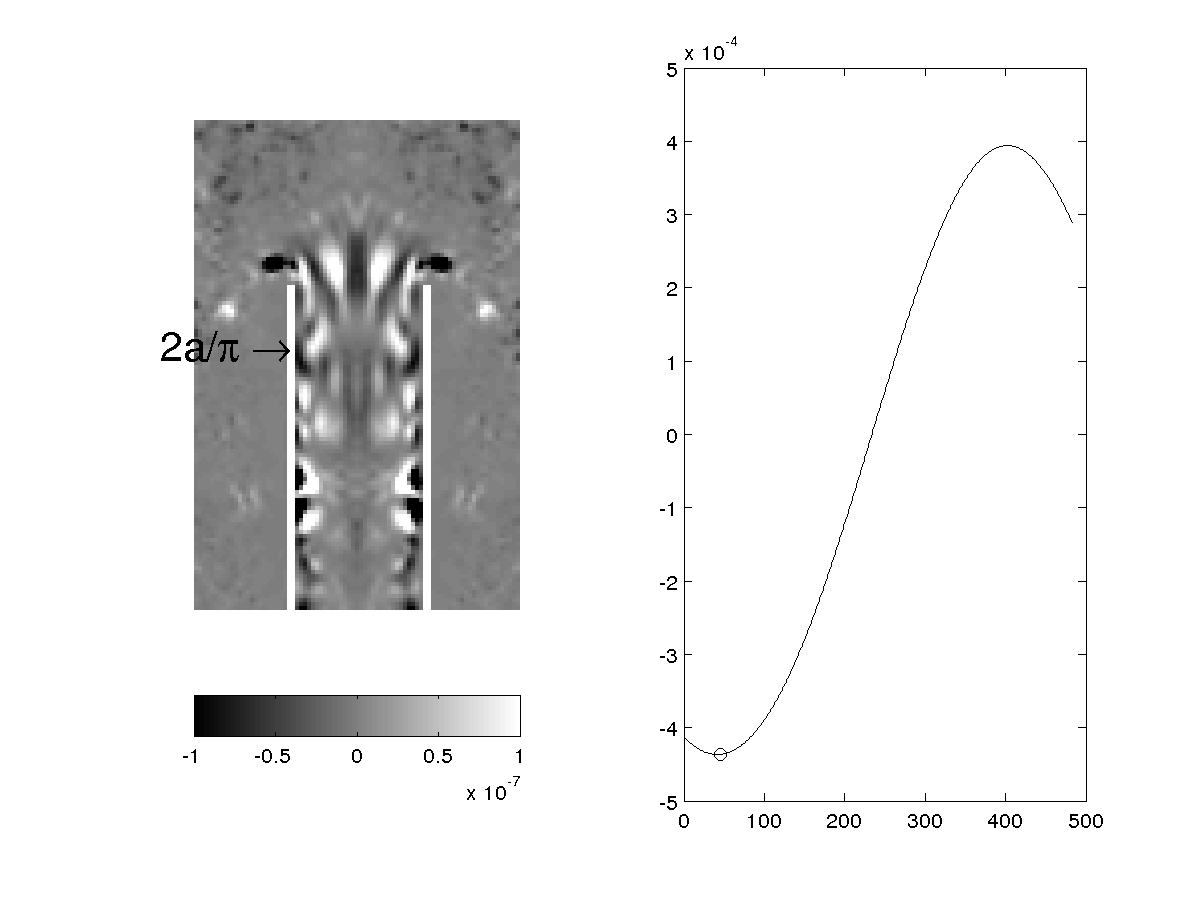
\includegraphics[width=1.\linewidth]{figuras/max_007_1.png}
  \caption[]{}
  \label{fig:max_007_1}
\end{subfigure}\par\medskip
\begin{subfigure}{0.9 \textwidth}
  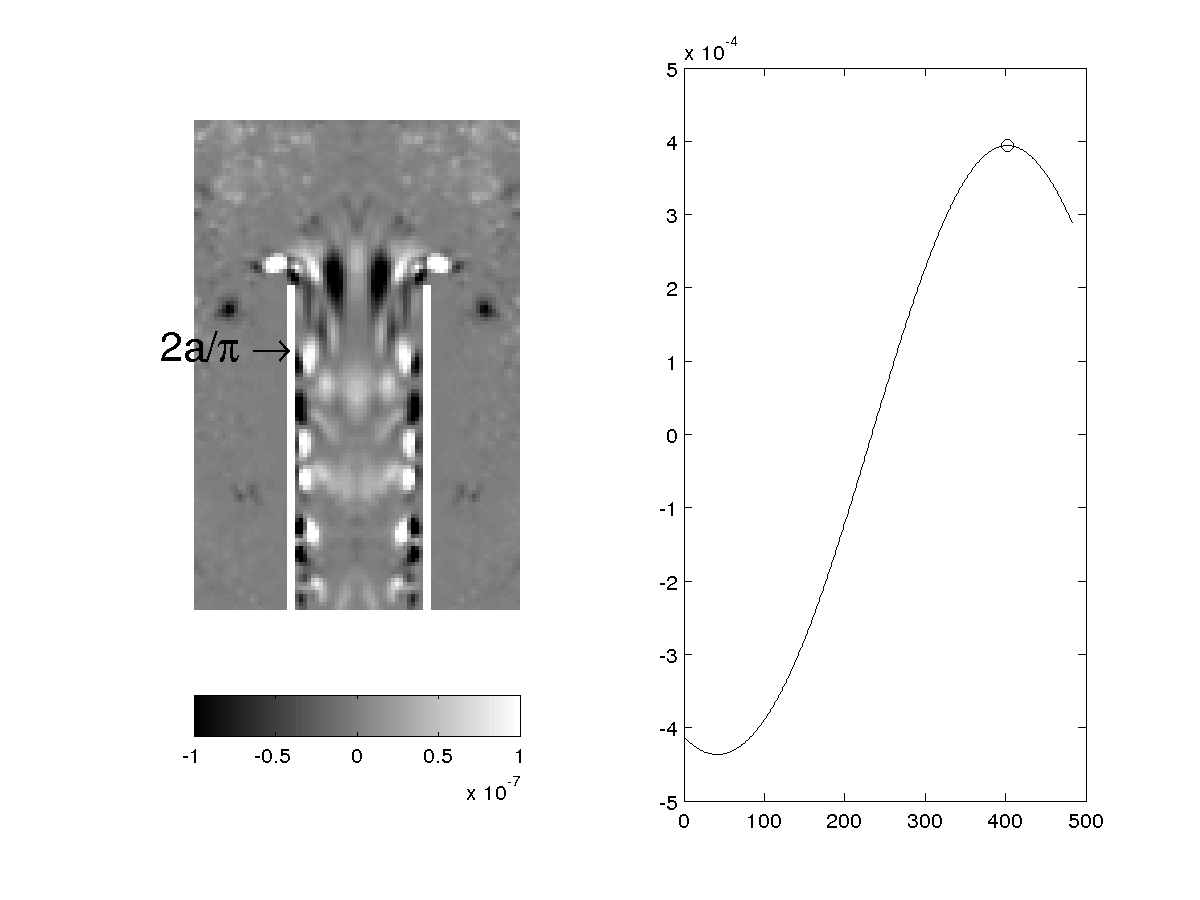
\includegraphics[width=1.\linewidth]{figuras/max_007_3.png}
  \caption[]{}
  \label{fig:max_007_3}
\end{subfigure}\par\medskip
\caption[Energia acústica para $M = 0,07$ e $St = \pi/2$.]{Energia acústica no interior do duto para $M = 0,07$ e $St = \pi/2$. A Figura \ref{fig:max_007_1} apresenta energia acústica no instante de vale da onda. A Figura \ref{fig:max_007_3} apresenta energia acústica no instante de crista da onda.}\label{fig:max_007}
\end{figure}

\vfill
\clearpage

\newpage
\vfill

 \begin{figure}[ht!]
 \begin{subfigure}{0.9 \textwidth}
   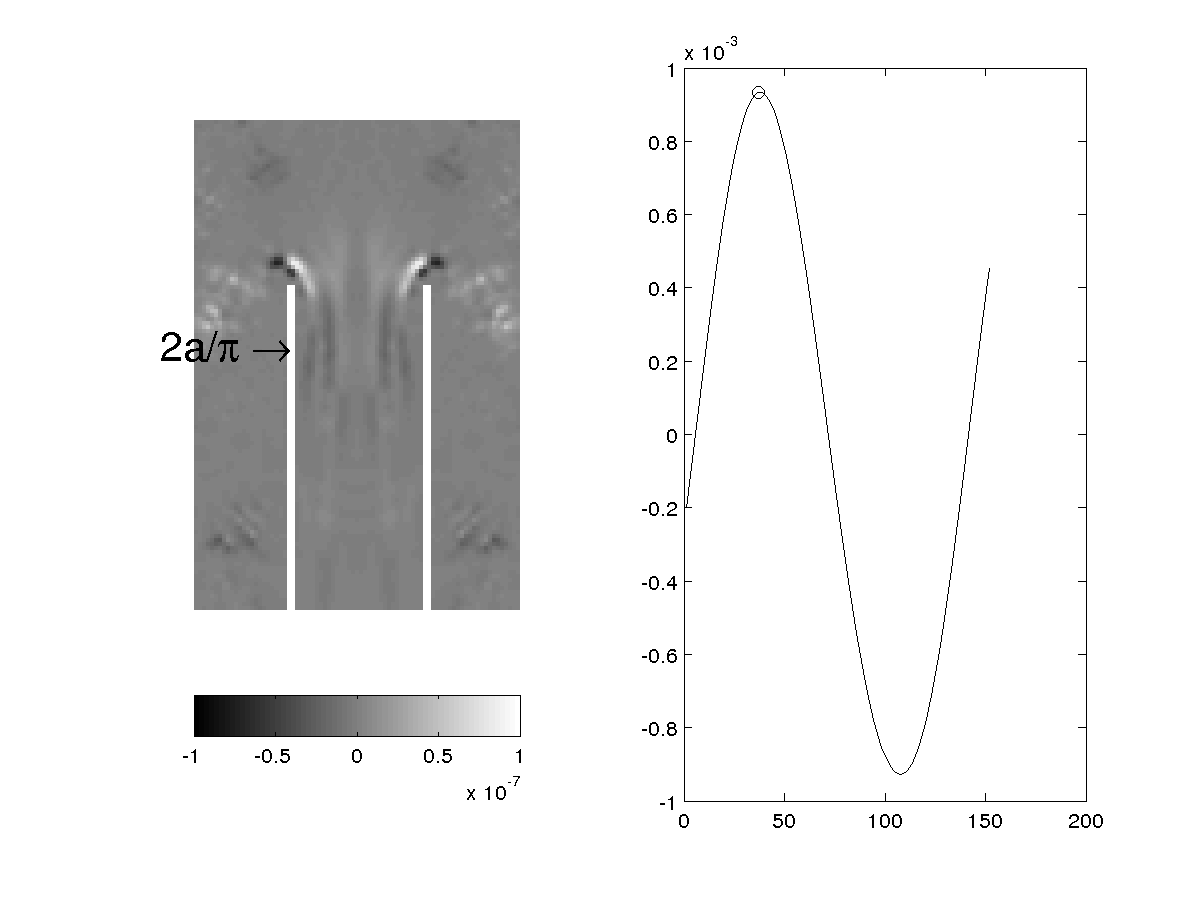
\includegraphics[width=1.\linewidth]{figuras/min_007_1.png}
   \caption[]{}
   \label{fig:min_007_1}
 \end{subfigure}\par\medskip
 \begin{subfigure}{0.9 \textwidth}
   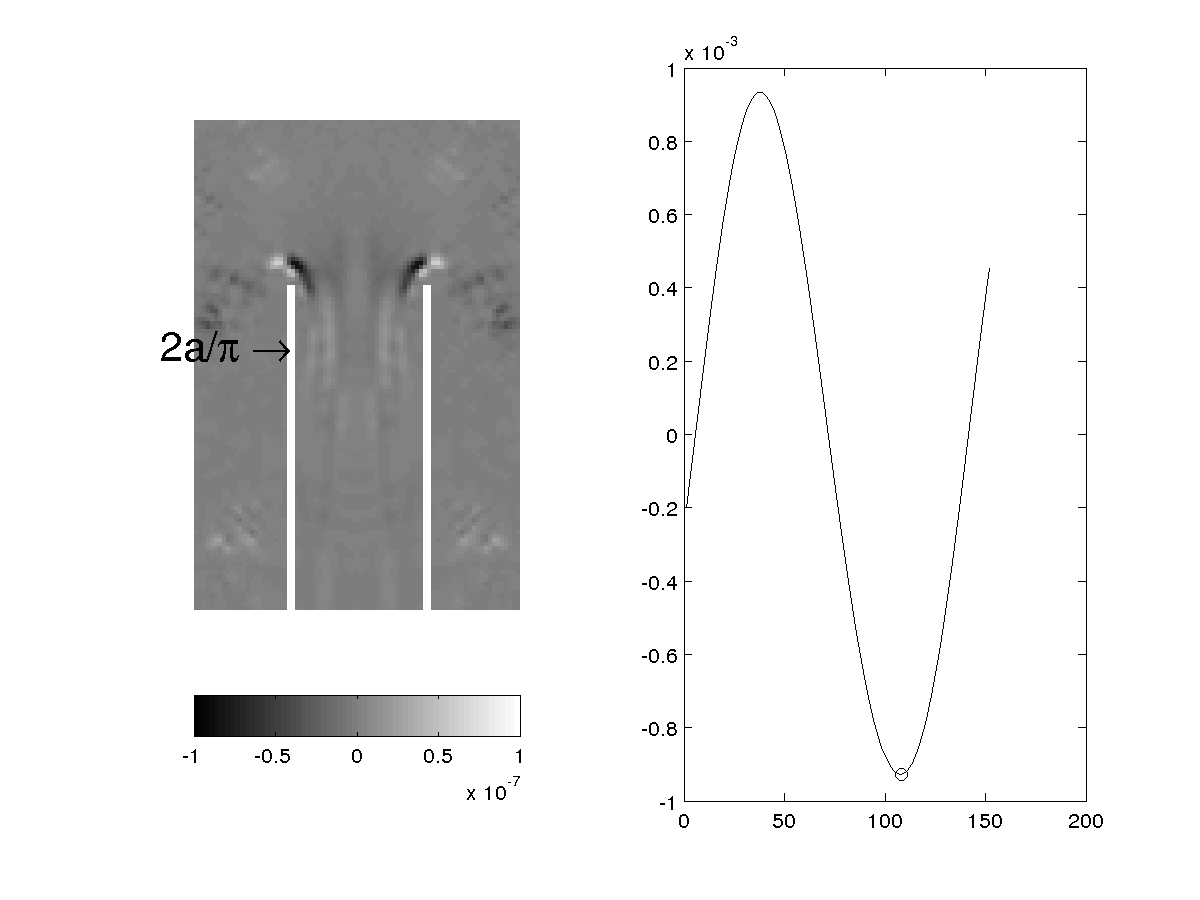
\includegraphics[width=1.\linewidth]{figuras/min_007_3.png}
   \caption[]{}
   \label{fig:min_007_3}
 \end{subfigure}\par\medskip
 \caption[Energia acústica para $M = 0,07$ e $St = 6,8$.]{Energia acústica no interior do duto para $M = 0,07$ e $St = 6,8$. A Figura \ref{fig:min_007_1} apresenta energia acústica no instante de crista da onda. A Figura \ref{fig:min_007_3} apresenta energia acústica no instante de vale da onda.}
 \label{fig:min_007}
 \end{figure}

\vfill
\clearpage

\newpage
\begin{figure}[ht!]
\centering
  \begin{tikzpicture}
  \begin{axis}[
  width=0.9\textwidth,
  height=0.5\textwidth,
  x tick label style={
      /pgf/number format/.cd,
          fixed,
          fixed zerofill,
          precision=2,
      /tikz/.cd
  },
  xmin=0.05,
  xmax=0.2,
  ymin=0.6826,
  ymax=1.1835,
  ytick distance=0.1,
  xtick distance=0.03,
  grid=major, % Display a grid  
  %grid style={dashed,gray!90}, % Set the style
  xlabel = $M$,
  ylabel = $|R_{r}|$,
  ]
 \addplot[color=black, thick] table[x index=0,y index=1] {dados/duto_sugado/abs_r_strouhal_mach.txt};

  \end{axis}
  \end{tikzpicture}
  \caption[Coeficiente de reflexão $R_{r}$ com escoamento de exaustão em relação ao número de Mach ($M$) no Strouhal $St = \pi/2$]{Resultado de magnitudes do coeficiente de reflexão $R_{r}$ fixados no Strouhal $St = \pi/2$ em relação ao número de Mach ($M$) para escoamentos sugados. Os resultados foram calculados no ponto $\textbf{P}$ na terminação do duto.}

  \label{fig:abs_r_sugado_strouhal_mach}
\end{figure}

Fixando o valor de Strouhal $St = \frac{\pi}{2}$ e analisando $|R_{r}|$ em relação aos números de Mach pode-se obter o comportamento do pico máximo de $|R_{r}|$ para cada número de Mach. A Figura \ref{fig:abs_r_sugado_strouhal_mach} apresenta esse resultado, mostrando um comportamento não monotônico, ou seja, $|R_{r}|$ se comporta de forma não regular a medida que o número de Mach aumenta. Tal fato é importante de se considerar pois difere significativamente do escoamento de exaustão. Vale ressaltar também que há um máximo em $M \sim 0,07$ e a medida que se aumenta o Mach além desse valor $|R_{r}|$ vai dimiuindo.

Tal fenômeno pode ser analisado e investigado através do colorário de Howe, calculando a potência acústica gerada para $M = 0,07$ e $M = 0,1$. A tabela \ref{table:potencia_mach} mostra esse procedimento fixando o número de Strouhal em $\pi/2$. Pode-se perceber que o fenômeno da amplificação é atenuado quando o número de Mach é maior que $0,07$.    

\begin{table}[ht!]
\centering
\caption{Potência acústica calculada ao longo de um período de onda para $St = \pi/2$ e diferentes números de Mach.}
\label{table:potencia_mach}
    \begin{tabular}{|l|l|l|l|}
        \hline
        $M$ & $<P>$ \\ \hline
        $0,07$ & 7.7594e-09  \\ \hline  
        $0,1$ & 4.3443e-09 \\ \hline
    \end{tabular}
\end{table}

A Figura \ref{fig:max_01_1} apresenta a energia acústica para $M = 0,1$ e $St = \pi/2$ no instante de vale de onda. É perceptível o surgimento do vórtice de amplificação do campo acústico, assim como ocorre na Figura \ref{fig:max_007_1}.

\begin{figure}[ht!]
\centering
  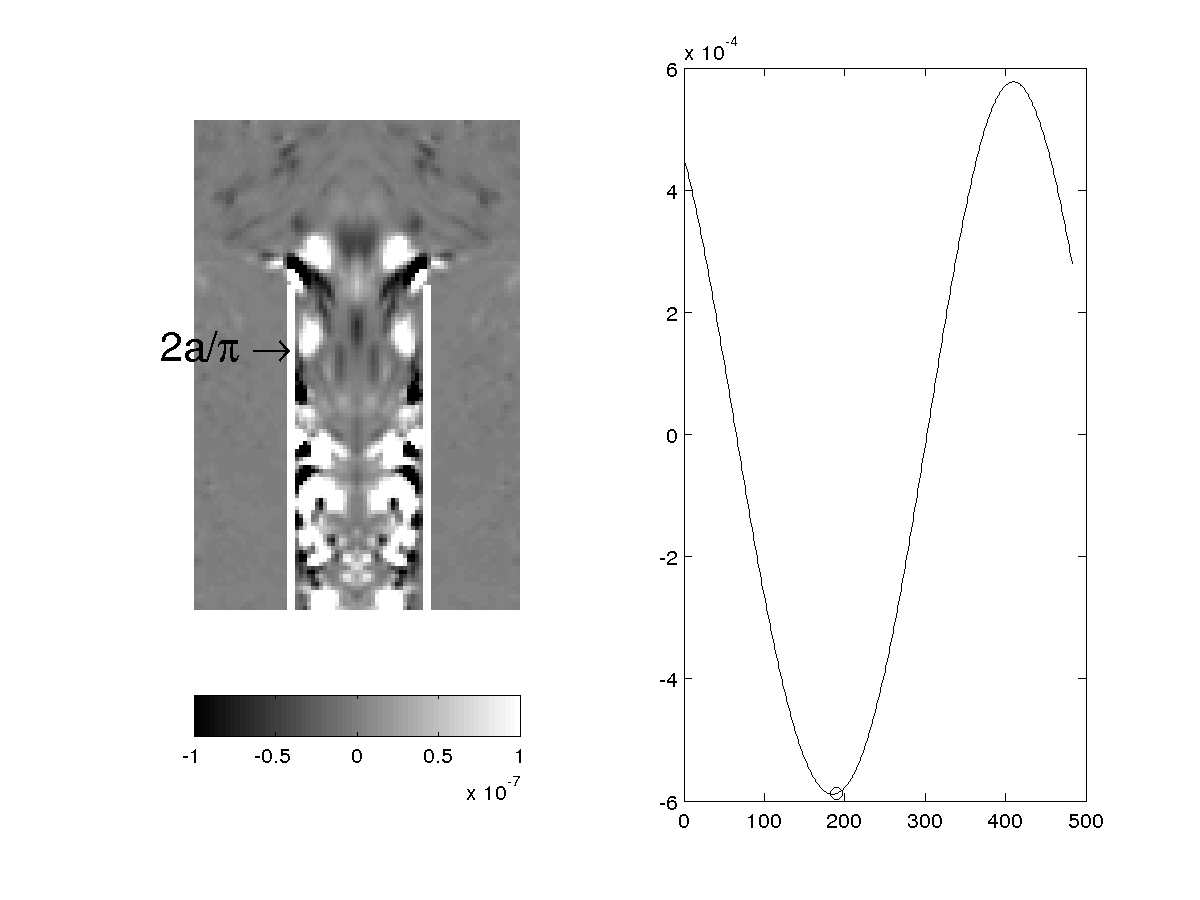
\includegraphics[width=1.\linewidth]{figuras/max_01_1.png}
  \caption[Energia acústica para $M = 0,1$ e $St = \pi/2$ no instante de vale de onda.]{Energia acústica para $M = 0,1$ e $St = \pi/2$ no instante de vale de onda.}
  \label{fig:max_01_1}
\end{figure}

A Figura \ref{fig:max_01_3} apresenta a energia acústica para $M = 0,1$ e $St = \pi/2$ no instante de crista de onda. Há um fenômeno que difere do caso da Figura \ref{fig:max_01_3}, há a apresença de desprendimento de vórtice com absorção de energia acústica. Esse vórtice se desprende da terminação e alcança a distância de $2a/\pi$. Tal fato é responsável pelo declínio e não monotonocidade do gráfico da Figura \ref{fig:abs_r_sugado_strouhal_mach} e estima-se que o vórtice aumenta de energia com o aumento da velocidade de escoamento e, consequentemente, aumentando a absorção do campo acústico.   

\newpage
\begin{figure}[ht!]
\centering
  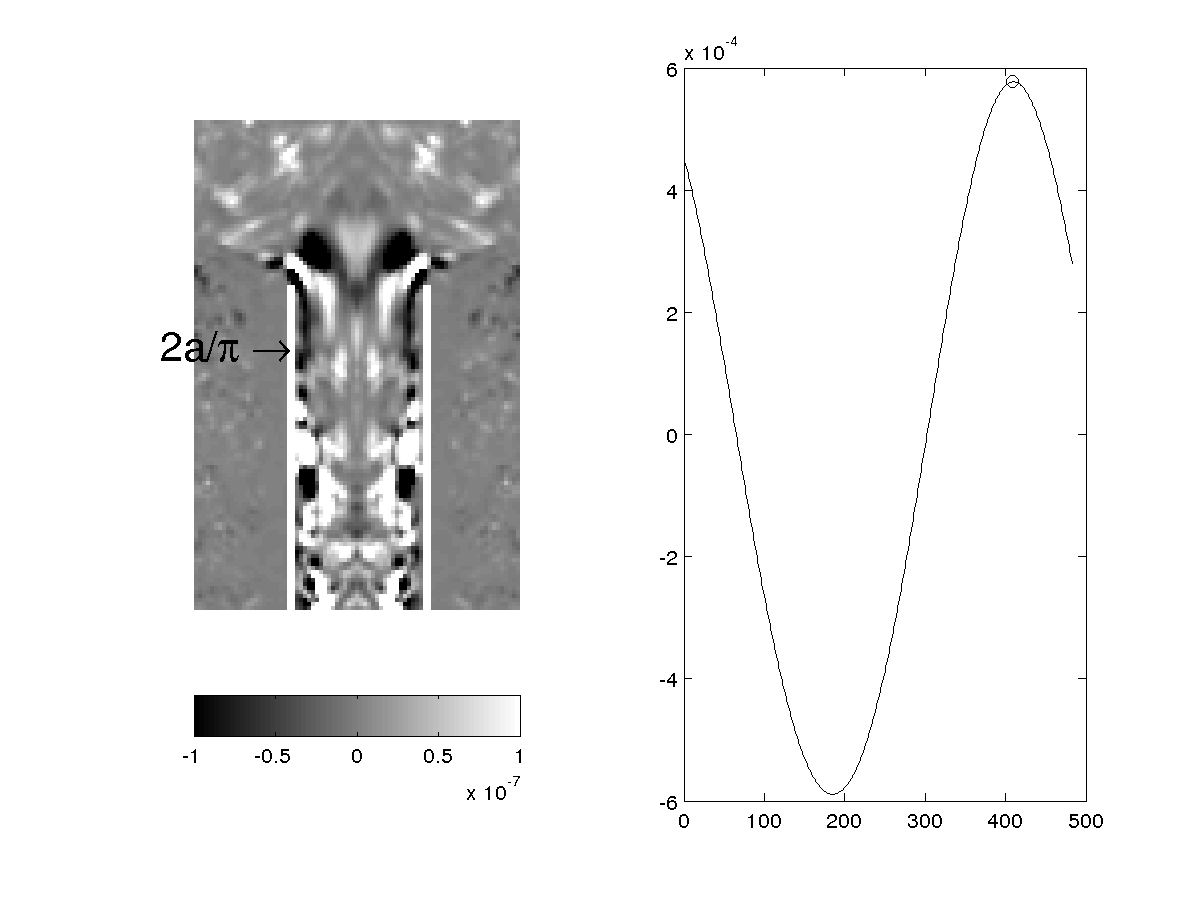
\includegraphics[width=1.\linewidth]{figuras/max_01_3.png}
  \caption[Energia acústica para $M = 0,1$ e $St = \pi/2$ no instante de vale de onda.]{Energia acústica para $M = 0,1$ e $St = \pi/2$ no instante de vale de onda.}
  \label{fig:max_01_3}
\end{figure}


%\newpage
%\begin{figure}[ht!]
%\centering
  %\begin{tikzpicture}
  \begin{axis}[
  width=0.9\textwidth,
  height=0.5\textwidth,
  x tick label style={
      /pgf/number format/.cd,
          fixed,
          fixed zerofill,
          precision=2,
      /tikz/.cd
  },
  xmin=0.05,
  xmax=0.2,
  ymin=0.,
  ymax=0.7,
  ytick distance=0.1,
  xtick distance=0.03,
  grid=major, % Display a grid  
  %grid style={dashed,gray!90}, % Set the style
  xlabel = $M$,
  ylabel = $l/a$,
  ]
 \addplot[color=black, thick] table[x index=0,y index=1] {dados/duto_sugado/loa_strouhal_mach.txt};

  \end{axis}
  \end{tikzpicture}
  \caption[Coeficiente de correção da terminação $l/a$ com escoamento de exaustão em relação ao número de Mach ($M$) no Strouhal $St = \pi/2$]{Resultado de coeficientes de correção da terminação $l/a$ fixados no Strouhal $St = \pi/2$ em relação ao número de Mach ($M$) para escoamentos sugados. Os resultados foram calculados no ponto $\textbf{P}$ na terminação do duto.}

  \label{fig:loa_sugado_strouhal_mach}
%\end{figure}

%valores de perda de carga:
%0.05 = 0.49
%0.07 = 0.59
%0.1 = 0.71
%0.15 = 0.74
%0.2 = 0.75

\chapter{Conclusões}

Nesse trabalho foi desenvolvida uma ferramenta computacional para análise do coeficiente de reflexão para modos normais em dutos na presença de escoamentos de baixo número de Mach ($M \leq 0,2$). 

Foi implementado um esquema computacional para avaliação do coeficiente de reflexão em dutos a partir do método de \textit{lattice} Boltzmann. Esse esquema foi desenvolvido em C++ orientado a objetos dentro do \textit{software} Palabos e fez uso do modelo MRT, condição de contorno de paredes rígidas e condição de contorno de absorção de energia acústica adaptada ao MRT. Os resultados mostraram que o esquema computacional funciona de acordo com os resultados da literatura e que a condição de absorção de energia acústica se comporta aproximadamente como impedância do meio.

Condições de contorno necessárias foram construídas, afim de representar o problema da reflexão de onda em dutos na presença de baixos números de Mach. As condições de contorno foram aplicadas num modelo numérico tridimensional de um duto não flangeado com espessura de paredes de $10 \%$ do tamanho do raio do duto. Além disso foram adaptadas as distâncias necessárias dos limites do domínio numérico em relação ao duto para que haja conservação da massa e que a condição de contorno de absorção possa se comportar regularmente. Os resultados mostraram que o modelo numérico é estável e representa o comportamento físico esperado num regime de baixos números de Mach.

Foi implementado, validado e analisado o comportamento acústico interno de dutos não flangeados com e sem escoamento de exaustão e com ondas planas. Os coeficientes de reflexão e de correção da terminação foram extraídos do modelo numérico com rotinas de pós-processamentos. Os mesmos foram comparados e analisados e possuem uma correlação em média de 90\%  com os resultados da litetura, demonstrando boa concordância com os fenômenos físicos abordados na litetura. Houve algumas divergências no coeficiente de correção da terminação num regime de exaustão e podem ser explicadas pelo fato do método de cálculo do pós-processamento não considerar a presença de escoamentos.  

O comportamento acústico interno de dutos não flangeados com escoamento sugado e com ondas planas foi implementado, validado e analisado. Os coeficientes de reflexão e de correção da terminação foram extraídos e pós-processados do modelo numérico num regime de escoamento sugado e comparado com os dados disponíveis na litetura. Apesar do coeficiente de correção da terminação não ter tido uma boa correlação, o coeficiente de reflexão foi calculado com 98,35\% de correlação demonstrando uma boa concordância com os dados da literatura. Apesar da literatura ter somente disponíveis resultados em baixas frequências ($ka \leq 0,25$) para escoamento sugado, foram calculados e analisados coeficientes de reflexão para vários números de Mach em médias e altas frequências ($ka > 0,25$). As análises demonstraram que o coeficiente de reflexão num contexto de escoamento sugado é altamente sensível a diferentes números de Mach, havendo sobretudo amplificação acima da faixa unitária para números de Strouhal $St \sim \frac{\pi}{2}$. Esse fenômeno pode ser explicado pelo fato do campo fluido dinâmico interagir com o campo acústico através de desprendimento de vórtices. Vale ressaltar também que a variação do coeficiente de reflexão em relação a vários Machs em $St \sim \frac{\pi}{2}$, diferentemente do que ocorre em regime de escoamento de exaustão que é monotônico, varia de forma não monotônica e possui um máximo em $M \sim 0,07$. Esse fenômeno pode ser explicado pela natureza do desprendimento de vórtices numa vena contracta.  


%%%%%%%%%%%%%%%%%%%%%%%%%%%%%%%%%%%%%%%%%%%%%%%%%%%%%%%%%%%%%%%%%%%%%%%%%


\bibliographystyle{ufscThesis/ufsc-alf}
\bibliography{bibliografia}
%%%%%%%%%%%%%%%%%%%%%	REFERÊNCIAS    %%%%%%%%%%%%%%%%%%%%%%%%%%%%%%%%%%%

%--------------------------------------------------------
% Elementos pós-textuais
\apendice
\chapter{Manual de Funcionamento do Palabos Acoustic}

Para executar o \citeonline{palabos_acoustic} é preciso dos seguintes \textit{softwares} básicos instalados como pré-requisitos:

\begin{itemize}
  \item sistema operacional linux Ubuntu 16.04 ou CentOS 7.2;
  \item compilador de C++ do tipo g++ 4.8;
  \item biblioteca de processamento paralelo Open MPI 1.10. 
\end{itemize}

Para cada novo modelo é preciso criar uma pasta com o nome do modelo contendo o arquivo de compilação \textbf{Makefile} e o código fonte do modelo numérico escrito em C++ com extenção \textbf{.cpp}. No arquivo \textbf{Makefile} é possível configurar aonde se encontra a instalação do Palabos, arquivo do modelo numérico com extenção \textbf{.cpp}, opções de depuração e opções de paralelização. No arquivo de extenção \textbf{.cpp} se encontra o código fonte do modelo numérico a ser simulado e o mesmo é composto de acordo com os procedimentos do fluxograma da Figura \ref{fig:palabos_fluxo}.


\begin{figure}[ht!]
\centering
  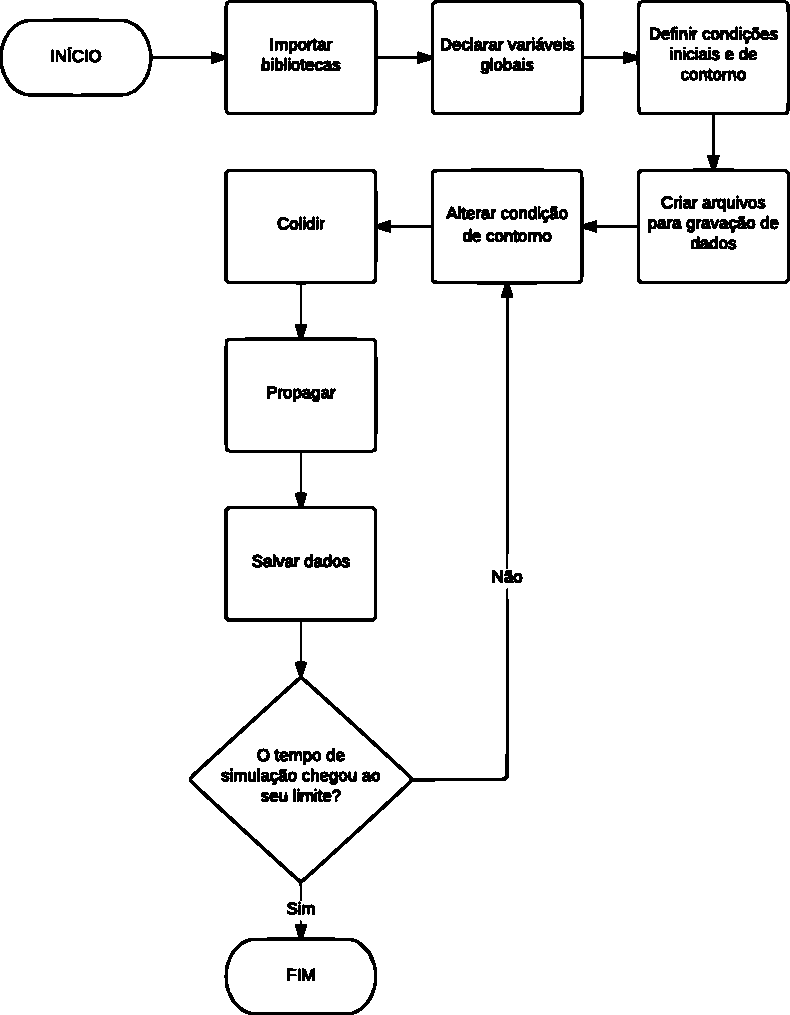
\includegraphics[width=.8\linewidth]{figuras/palabos_modelo_fluxo.pdf}
  \caption[Fluxograma de um modelo numérico no Palabos]{Fluxograma geral de um código fonte de um modelo numérico no Palabos.}
  \label{fig:palabos_fluxo}
\end{figure}

Como é mostrado na Figura \ref{fig:palabos_fluxo}, todo código de modelo numérico no Palabos possui os seguintes procedimentos:

\begin{itemize}
  \item importar bibliotecas: nesse procedimento são importadas as bibliotecas que contêm as funções e classes que serão usadas ao longo do processamento do modelo. Normalmente são bibliotecas do próprio Palabos ou bibliotecas com funções matemáticas;
  \item definir variáveis globais: normalmente nessa etapa são definidas valores de pré-processamento como o tamanho do domínio, valores macroscópicos do fluido como número de Reynolds, tempo total de simulação, viscosidade cinemática e o tipo de modelo LBM;
  \item definir condições iniciais e de contorno: nessa etapa a malha do domínio é consolidada, valores de densidade e velocidade são atribuídas para cada célula do domínio e condições de contorno são impostas;
  \item criar arquivos para gravação de dados: são criados ponteiros e arquivos de diversas extensões para que os dados sejam gravados;
  \item alterar condição de contorno: nessa etapa o modelo numérico entra no \textit{loop} de iterações e se necessário as condições de contorno são alteradas para, por exemplo, que um \textit{sweep} possa ser imposto;
  \item colidir: nessa etapa o operador de colisão é calculado e somado com as funções de distribuição de cada célula;
  \item propagar: os valores das funções de distribuição são propagados para células vizinhas;
  \item salvar dados: os dados normalmente de pressão e velocidades são salvos para pós-processamento. 
\end{itemize}
E assim o ciclo de procedimentos dentro do \textit{loop} é executado até que o número de iterações alcance o número máximo de tempo definido no início do programa.

Para execução é preciso efetuar os seguintes comandos no terminal linux dentro da pasta do modelo numérico:
\begin{itemize}
  \item compilação do código de extenção \textbf{.cpp} para formato binário em linguagem de máquina:
  \begin{lstlisting}[language=make, frame = single]
    $ make
  \end{lstlisting}
  \item execução do arquivo binário compilado:
  \begin{lstlisting}[language=make, frame = single]
    $ mpirun -np 
    <numero_de_processadores> 
    <nome_do_arquivo_compilado> 
    <parametros_de_entrada>
  \end{lstlisting}
  aplicando para o modelo numérico desse trabalho:
  \begin{lstlisting}[language=make, frame = single]
    $ mpirun -np 
    8
    duct_radiation_optimization
    20 0.15 1.99
  \end{lstlisting}
  tal que o raio do duto é 20 células, o mach do escoamento é 0.15 e 1.99 é a frequência de relaxação $1/\tau$. É possível também executar o Palabos com o \textit{script} \textbf{duct\_radiation\_init.m} na plataforma \citeonline{matlab} ou \citeonline{octave}. Para executar basta colocar esse \textit{script} dentro da pasta do modelo numérico e executar o seguinte comando no terminal do \citeonline{matlab} ou \citeonline{octave} dentro dessa pasta:
  \begin{lstlisting}[language=matlab, frame = single]
    >> duct_radiation_init 20 0.15 5042 8
  \end{lstlisting}
  tal que o raio do duto é 20 células, o mach do escoamento é 0.15, o número de Reynolds é 5042 e o 8 é a quantidade de processadores.
\end{itemize}


%\anexo
%\chapter{Exemplificando um Anexo}
%Texto do anexo aqui.
\end{document}
